% Options for packages loaded elsewhere
\PassOptionsToPackage{unicode}{hyperref}
\PassOptionsToPackage{hyphens}{url}
%
\documentclass[
]{book}
\usepackage{amsmath,amssymb}
\usepackage{iftex}
\ifPDFTeX
  \usepackage[T1]{fontenc}
  \usepackage[utf8]{inputenc}
  \usepackage{textcomp} % provide euro and other symbols
\else % if luatex or xetex
  \usepackage{unicode-math} % this also loads fontspec
  \defaultfontfeatures{Scale=MatchLowercase}
  \defaultfontfeatures[\rmfamily]{Ligatures=TeX,Scale=1}
\fi
\usepackage{lmodern}
\ifPDFTeX\else
  % xetex/luatex font selection
\fi
% Use upquote if available, for straight quotes in verbatim environments
\IfFileExists{upquote.sty}{\usepackage{upquote}}{}
\IfFileExists{microtype.sty}{% use microtype if available
  \usepackage[]{microtype}
  \UseMicrotypeSet[protrusion]{basicmath} % disable protrusion for tt fonts
}{}
\makeatletter
\@ifundefined{KOMAClassName}{% if non-KOMA class
  \IfFileExists{parskip.sty}{%
    \usepackage{parskip}
  }{% else
    \setlength{\parindent}{0pt}
    \setlength{\parskip}{6pt plus 2pt minus 1pt}}
}{% if KOMA class
  \KOMAoptions{parskip=half}}
\makeatother
\usepackage{xcolor}
\usepackage{longtable,booktabs,array}
\usepackage{calc} % for calculating minipage widths
% Correct order of tables after \paragraph or \subparagraph
\usepackage{etoolbox}
\makeatletter
\patchcmd\longtable{\par}{\if@noskipsec\mbox{}\fi\par}{}{}
\makeatother
% Allow footnotes in longtable head/foot
\IfFileExists{footnotehyper.sty}{\usepackage{footnotehyper}}{\usepackage{footnote}}
\makesavenoteenv{longtable}
\usepackage{graphicx}
\makeatletter
\def\maxwidth{\ifdim\Gin@nat@width>\linewidth\linewidth\else\Gin@nat@width\fi}
\def\maxheight{\ifdim\Gin@nat@height>\textheight\textheight\else\Gin@nat@height\fi}
\makeatother
% Scale images if necessary, so that they will not overflow the page
% margins by default, and it is still possible to overwrite the defaults
% using explicit options in \includegraphics[width, height, ...]{}
\setkeys{Gin}{width=\maxwidth,height=\maxheight,keepaspectratio}
% Set default figure placement to htbp
\makeatletter
\def\fps@figure{htbp}
\makeatother
\setlength{\emergencystretch}{3em} % prevent overfull lines
\providecommand{\tightlist}{%
  \setlength{\itemsep}{0pt}\setlength{\parskip}{0pt}}
\setcounter{secnumdepth}{5}
\usepackage{booktabs}
\ifLuaTeX
  \usepackage{selnolig}  % disable illegal ligatures
\fi
\usepackage[]{natbib}
\bibliographystyle{plainnat}
\usepackage{bookmark}
\IfFileExists{xurl.sty}{\usepackage{xurl}}{} % add URL line breaks if available
\urlstyle{same}
\hypersetup{
  pdftitle={6ª EcoEscola: livro de resumos},
  hidelinks,
  pdfcreator={LaTeX via pandoc}}

\title{6ª EcoEscola: livro de resumos}
\author{}
\date{\vspace{-2.5em}2025-05-13}

\begin{document}
\maketitle

{
\setcounter{tocdepth}{1}
\tableofcontents
}
\chapter{Sobre}\label{sobre}

Este livro contém os resumos dos projetos realizados durante a 6ª EcoEscola

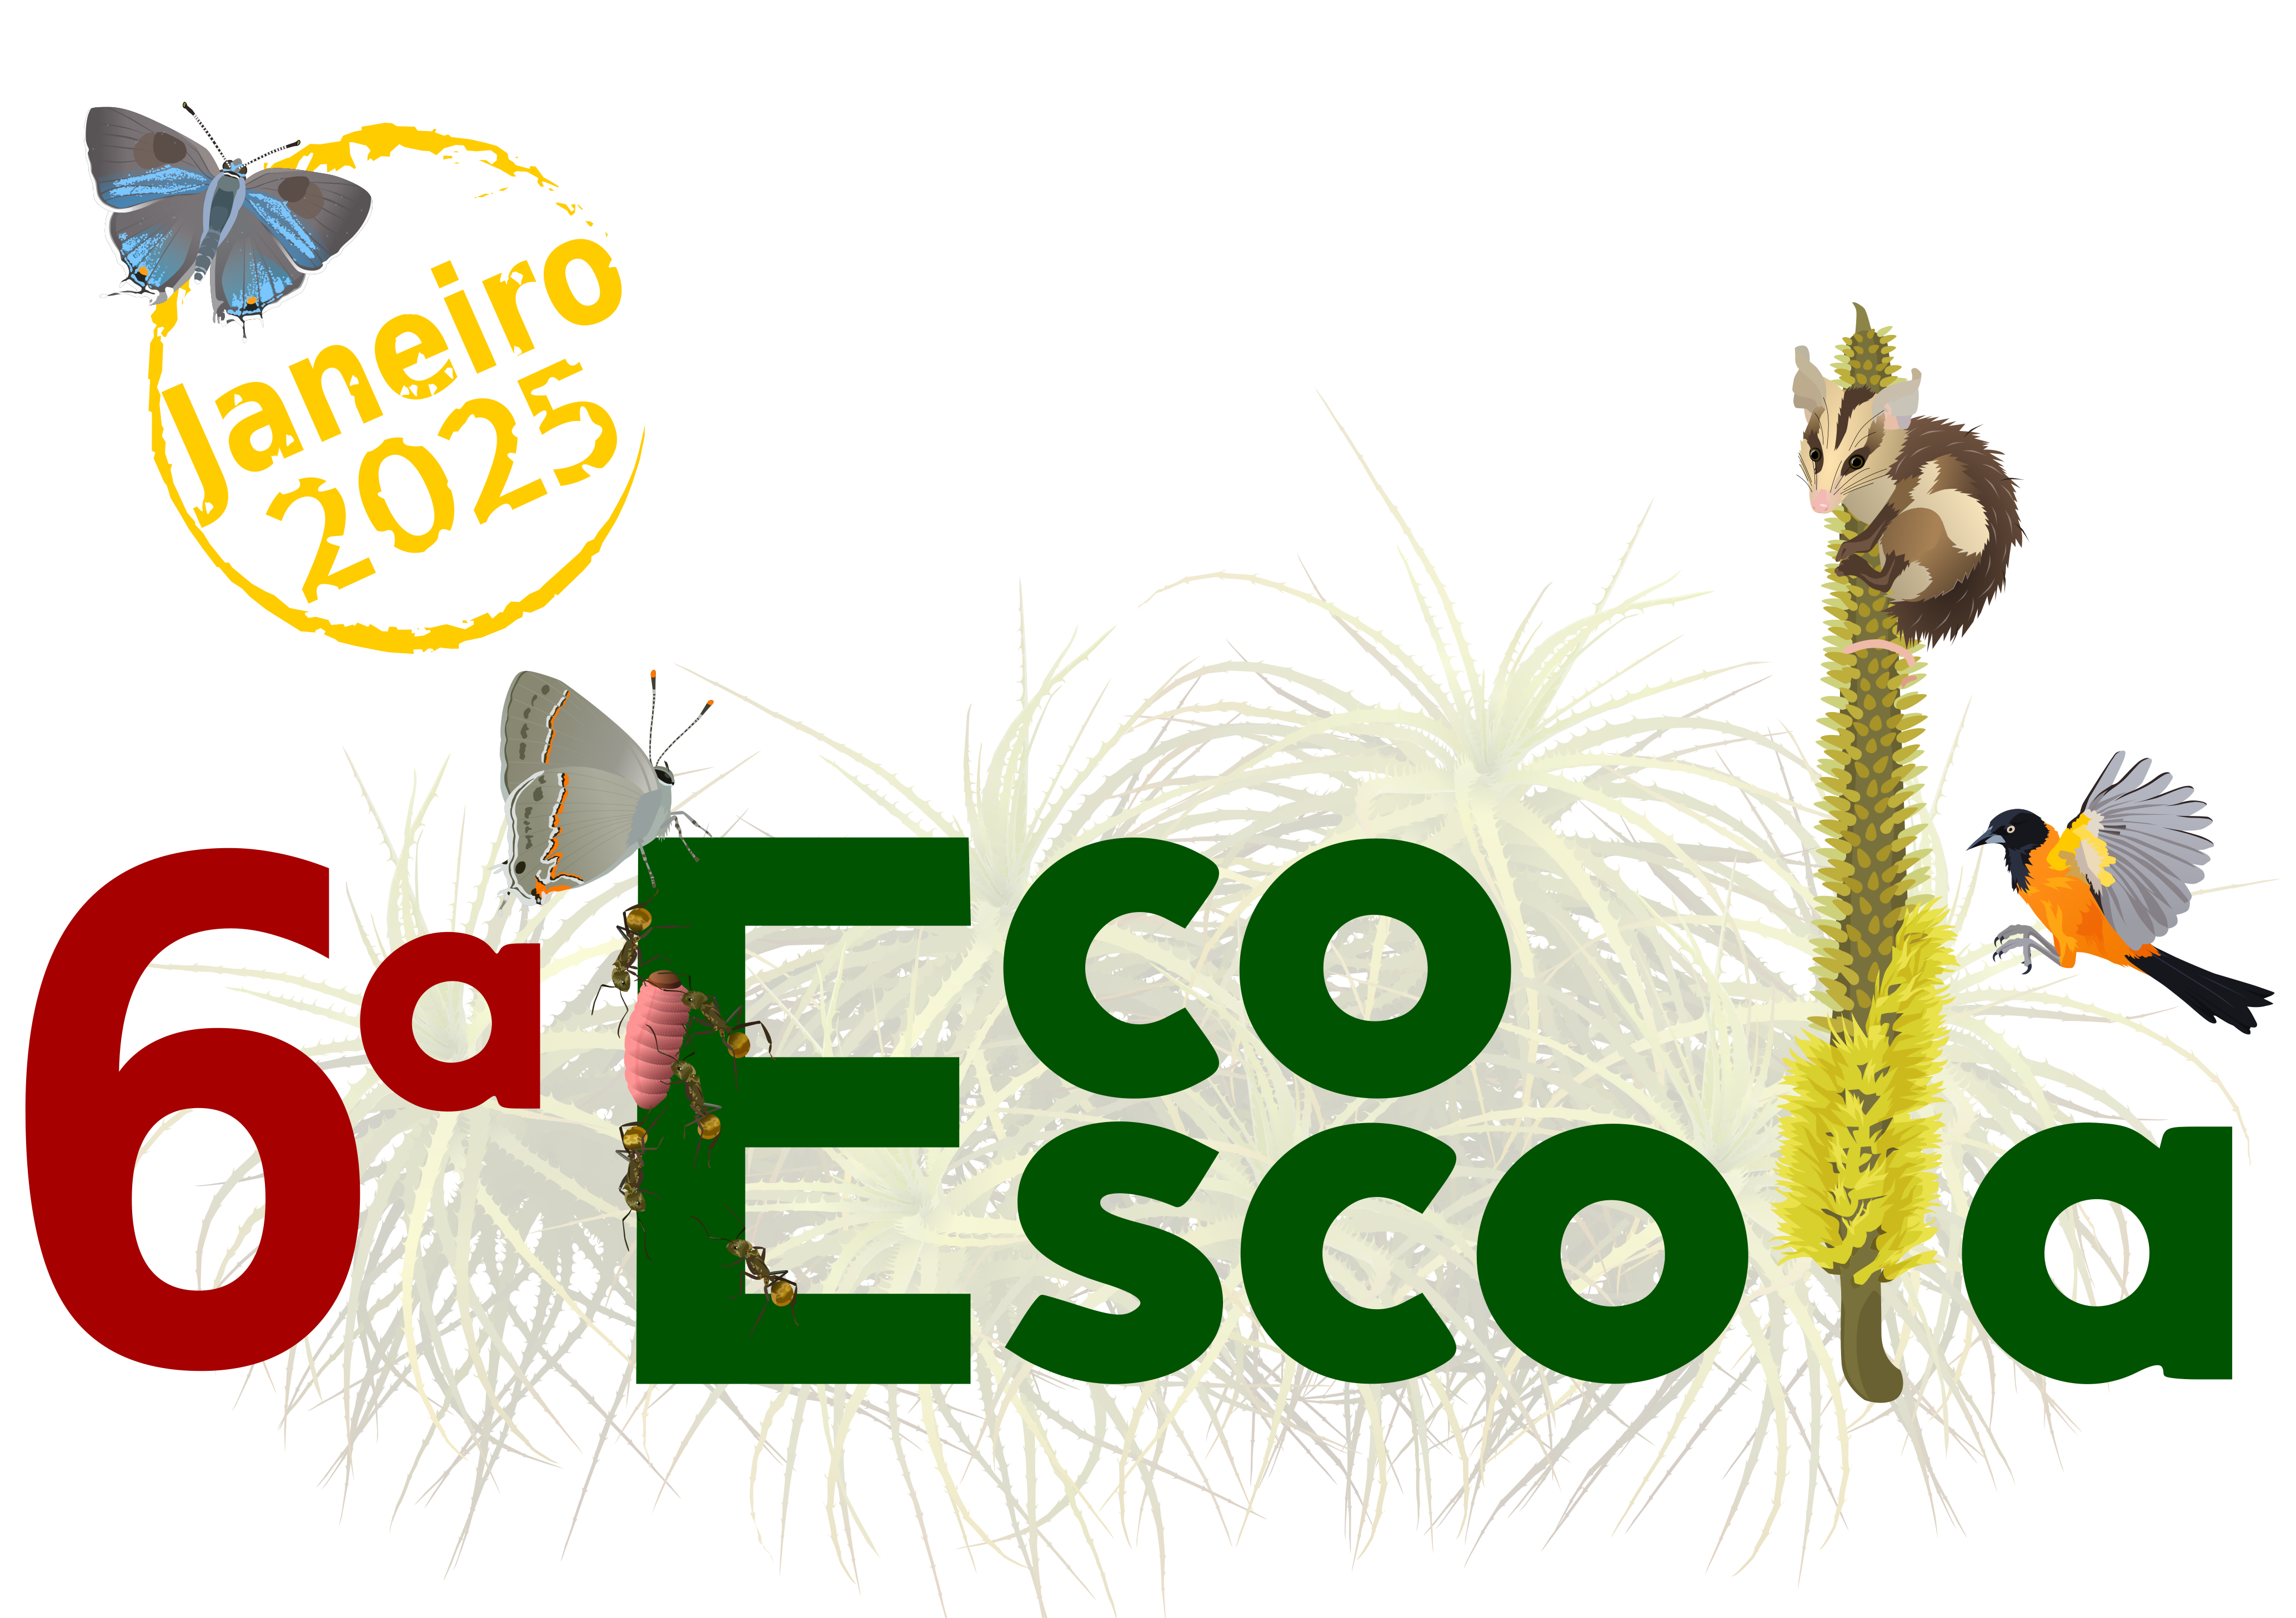
\includegraphics[width=57.42in]{figs/ecoescolalogo}

\chapter{Introdução}\label{introduuxe7uxe3o}

Este livro contém os resumos dos trabalhos realizados durante a 6ª EcoEscola.
Esta é a primeira iniciativa de organização dos resumos. Pretendemos que este
material sirva de duas formas. Para apresentar os projetos realizados durante
o módulo prático da EcoEscola, e que sirva como fonte de inspiração para projetos
rápidos (duas semanas) que envolvam coleta, análise e interpretação de dados.
Pretendemos que este material também sirva para professores e educadores de
ensino superior e médio para fornecer possíveis atividades práticas que possam
ser utilizadas em aulas de ensino de Ecologia para nível médio e superior.

\section{A EcoEscola}\label{a-ecoescola}

A Escola de Ecologia da USP (EcoEscola) é um curso teórico-prático de pesquisa em Ecologia, que abrange tópicos de ecologia geral e fundamentação da metodologia científica, sendo um evento totalmente organizado majoritariamente pelos alunos do Programa de Pós-Graduação em Ecologia da Universidade de São Paulo (PPGE-USP).

\section{Por que a EcoEscola não é só mais um curso teórico-prático em ecologia}\label{por-que-a-ecoescola-nuxe3o-uxe9-suxf3-mais-um-curso-teuxf3rico-pruxe1tico-em-ecologia}

Mais um curso de Ecologia? Os cursos que aliam teoria e prática em ecologia são comuns atualmente. A EcoEscola também visa oferecer tanto ensino quanto uma experiência de prática em pesquisa, porém, o diferencial é que o foco da EcoEscola não está apenas na formação de estudantes.

Desde o seu princípio a EcoEscola visa, além da formação de estudantes em estágios finais da graduação, a complementação da formação para professores de biologia da rede pública. Outro diferencial da EcoEscola é a possibilidade para que pós-graduandos possam adquirir experiência didática ao ministrar aulas. Para tanto, neste ano foi oferecido um workshop para introdução ao método de ensino por investigação, ministrado pela professora (Daniela Lopes Scarpa){[}{]}, proporcionando aos professores ministrantes uma base conceitual e prática para a elaboração de aulas que vão além da simples exposição de conteúdos e temas para os estudantes. As aulas são preparadas seguindo o método de ensino por investigação e a comissão organizadora participa ativamente na elaboração do plano de aula juntamente com os professores.

\section{Modulo teórico - ensino por investigação}\label{modulo-teuxf3rico---ensino-por-investigauxe7uxe3o}

O curso é dividido em dois módulos, teórico e prático. O primeiro módulo é composto por aulas práticas e expositivas, baseadas no método de ensino por investigação e aprendizagem ativa, com duração de 5 dias. As aulas são ministradas majoritariamente por estudantes e pós-doutorandos do PPG em Ecologia do IB-USP, abrangendo temas de ecologia de populações, comunidades, paisagem, ecologia comportamental, evolução e princípios de conservação. Ainda há uma palestra e um momento para apresentação das linhas de pesquisa do programa de pós-graduação em Ecologia da USP.

\begin{center}\includegraphics[width=0.9\linewidth]{figs/aula_modulo1} \end{center}

\section{Módulo 2 - Prática em ecologia}\label{muxf3dulo-2---pruxe1tica-em-ecologia}

O segundo módulo mescla uma semana de aulas com aprendizagem ativa. As aulas abrangem uma introdução ao método científico, com tópicos em ecologia como ciência, ferramentas de pesquisa bibliográfica, delineamento experimental e análise estatística. Após as aulas os estudantes tem duas semanas de atividades práticas dentro da universidade, buscando ensinar e aplicar os conceitos aprendidos através do desenvolvimento de um projeto de pesquisa em ecológica. Este projeto envolve todas as fases de uma pesquisa científica, desde o delineamento amostral, a coleta, análise de dados e apresentação dos resultados.

\begin{center}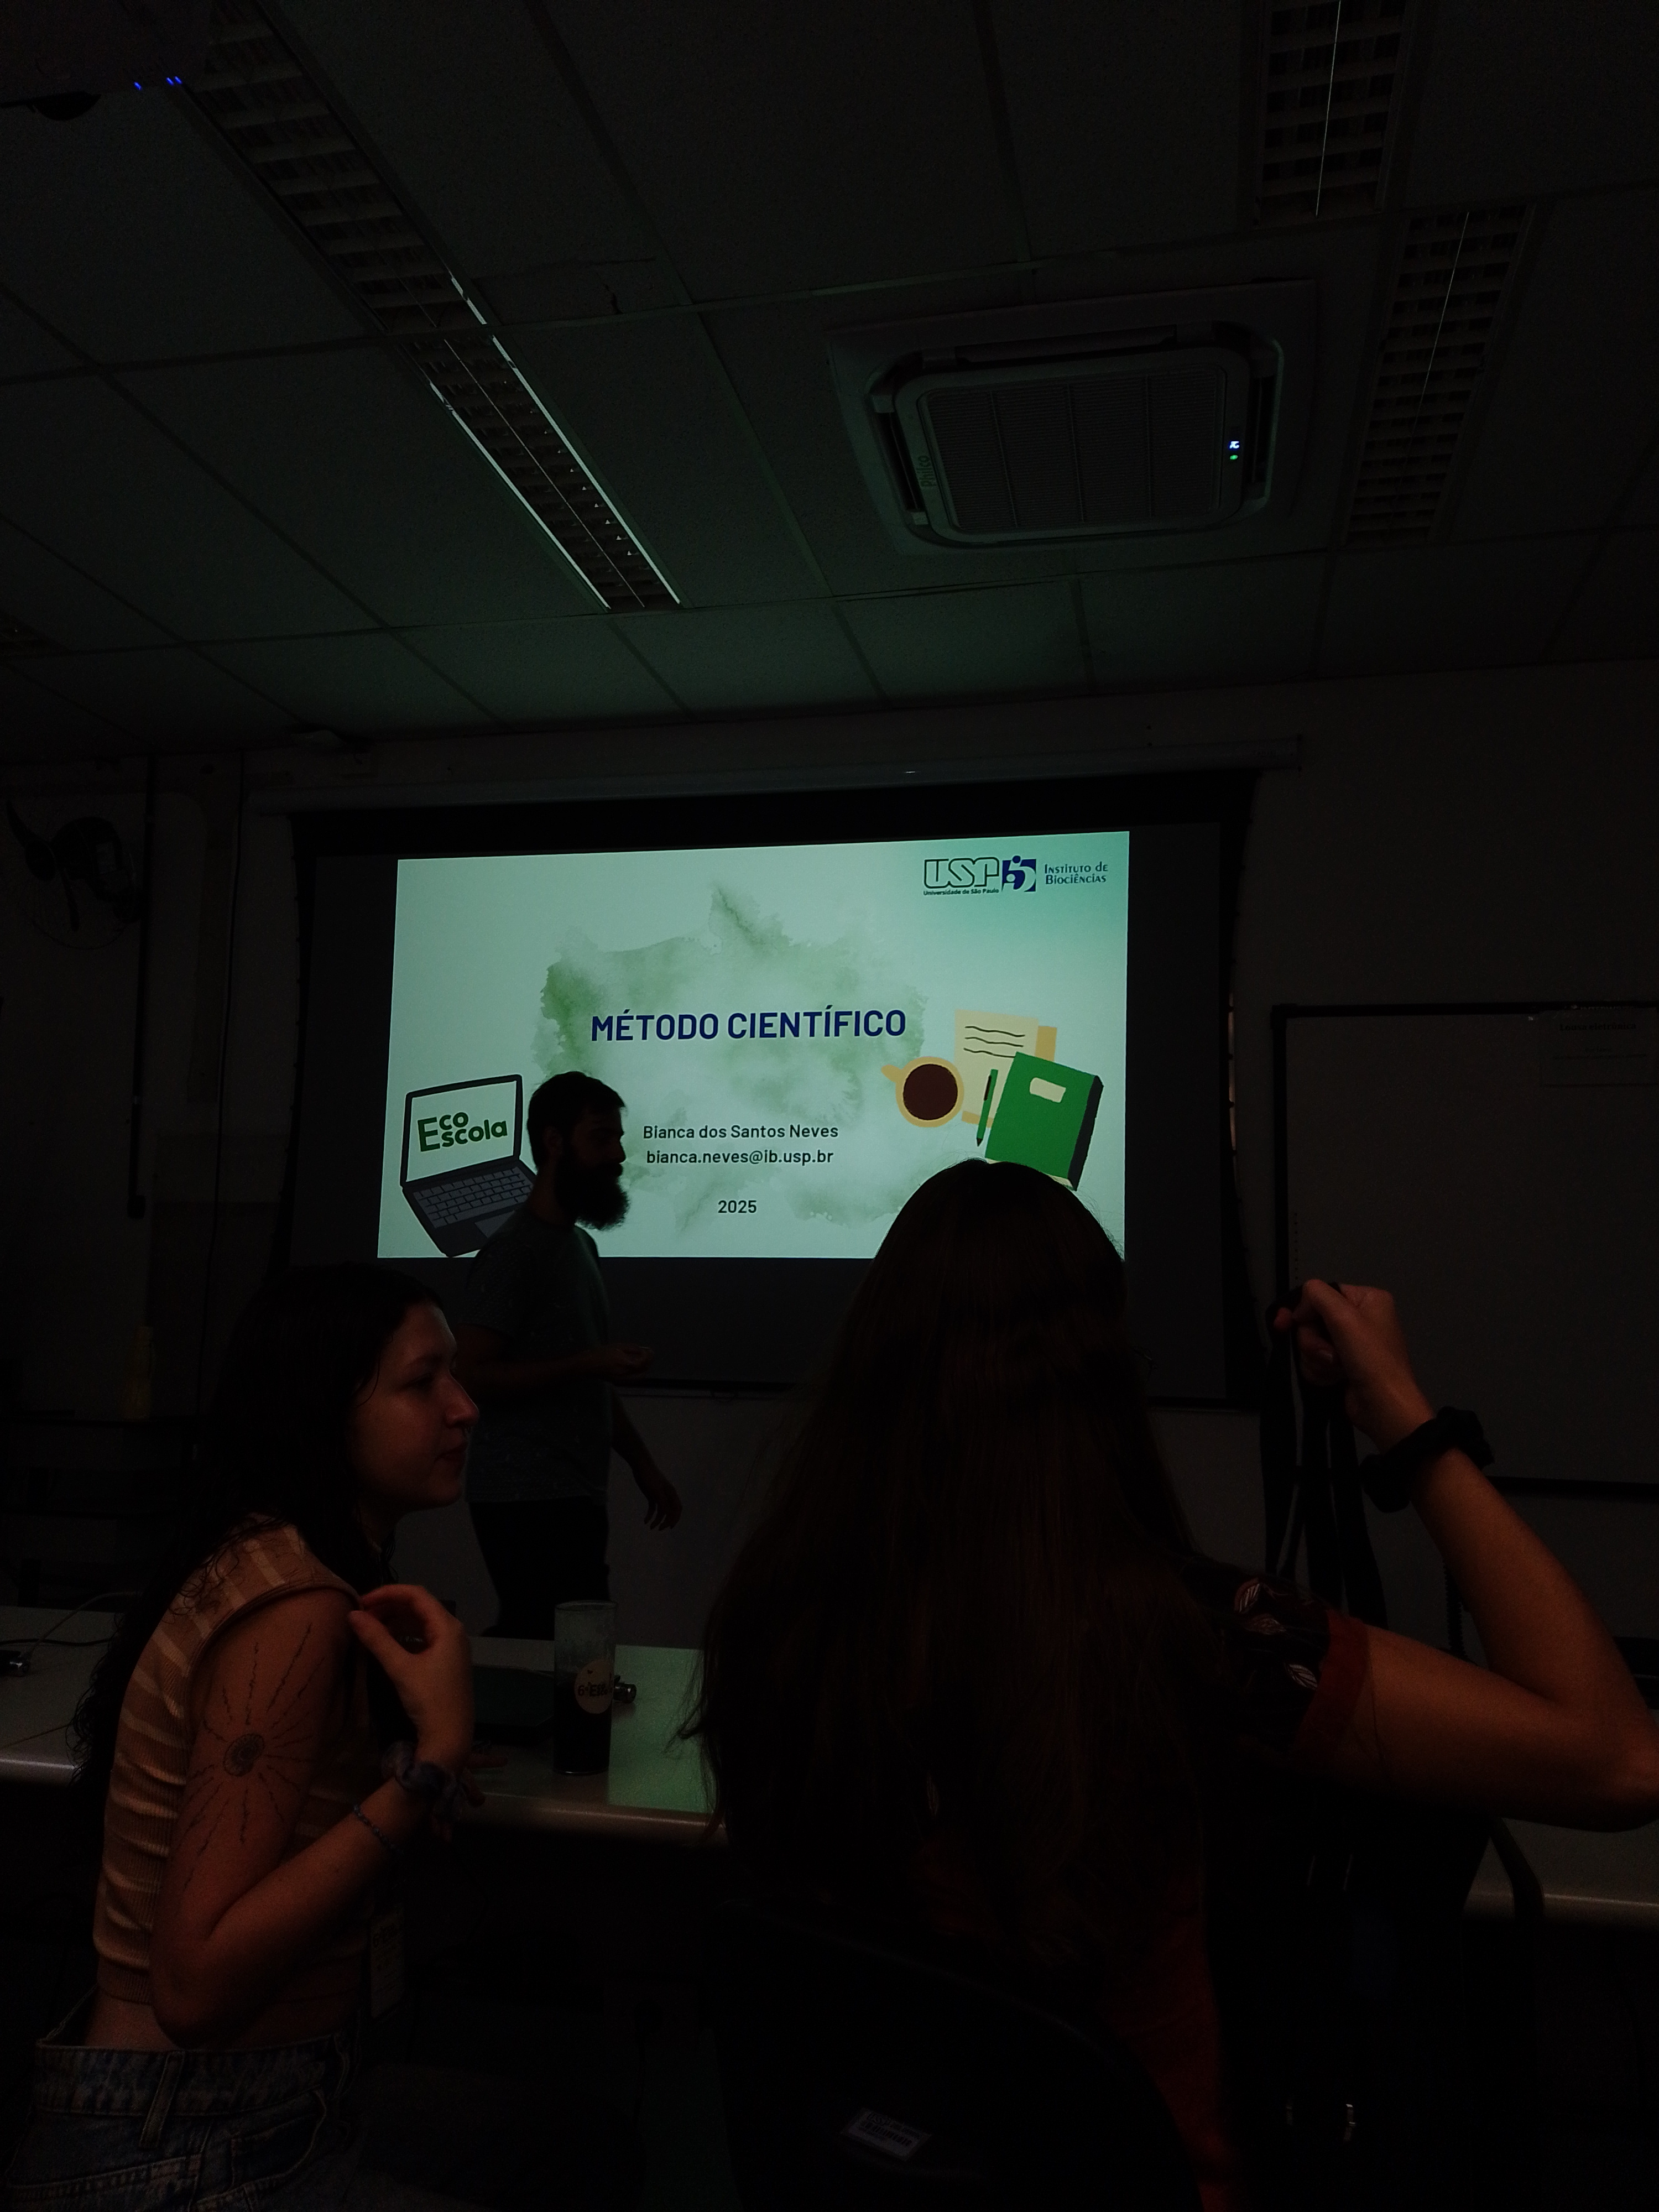
\includegraphics[width=0.9\linewidth]{figs/aula_modulo2} \end{center}

\section{Ensino por investigação}\label{ensino-por-investigauxe7uxe3o}

{[}textinho da Gabi{]}

\chapter{Organização}\label{organizauxe7uxe3o}

A EcoEscola só existe graças ao esforço coletivo e voluntário dos alunos da pós graduação em ecologia da Universidade de São Paulo. As três semanas de curso são resultado de um ano inteiro de programação realizada pela comissão da EcoEscola. Nesta 6ª edição o curso contou com 10 integrantes.

\begin{center}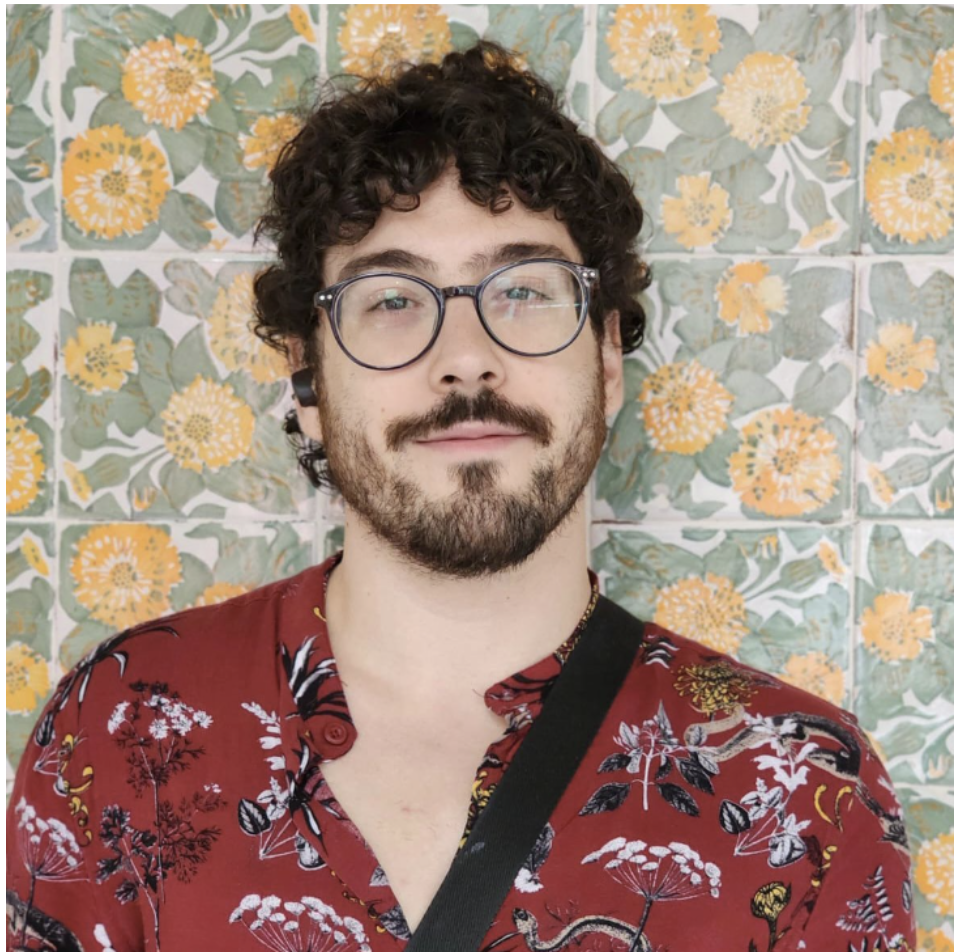
\includegraphics[width=0.5\linewidth]{figs/arthur_picture} \end{center}

\textbf{Arthur Lupinetti}

Doutorando e mestre em Ecologia no Laboratório de Ecologia e Conservação da USP, graduado em Ciências Biológicas e Engenharia Ambiental e Urbana na UFABC

\begin{quote}
``Participei como aluno da quarta EcoEscola, o que foi um grande incentivo para ingressar no mestrado em ecologia. Quando a organização da quinta edição iniciou, não tive duvida em participar da comissão''
\end{quote}

\begin{center}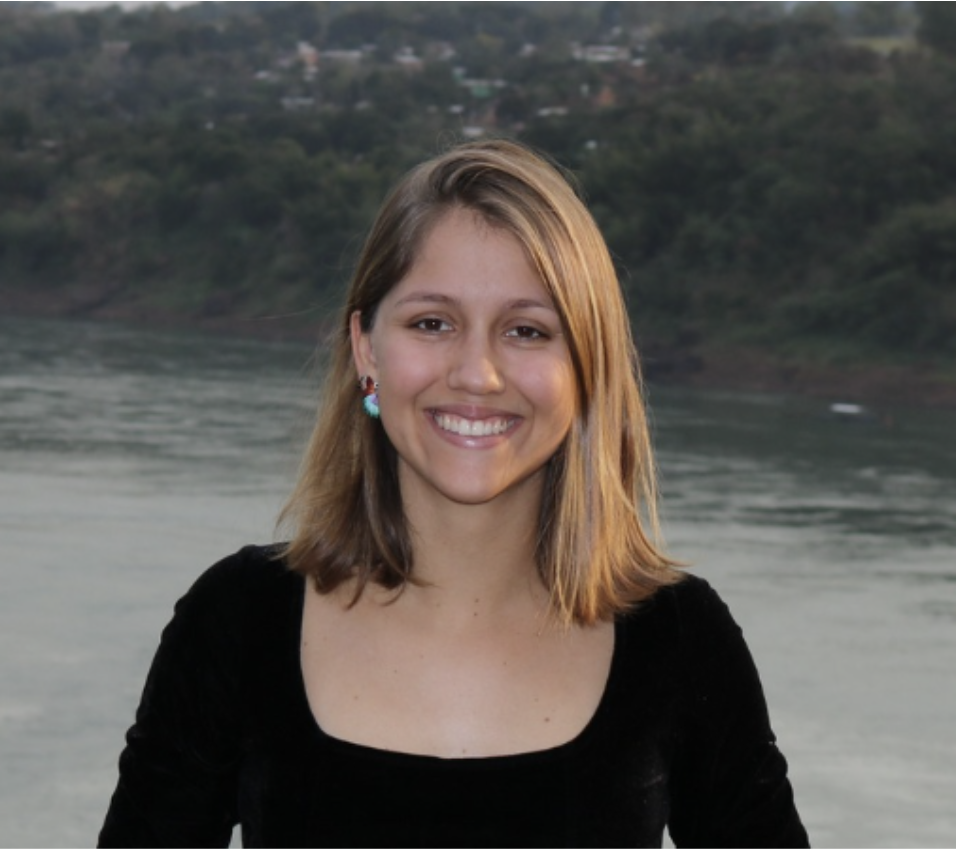
\includegraphics[width=0.5\linewidth]{figs/bianca_picture} \end{center}

\textbf{Bianca Neves}

Mestranda em Ecologia no Laboratório de Ecologia de Paisagem e Conservação na USP, fez graduação em Ciências Biológicas na UFES

\begin{quote}
``Conheci o projeto na minha semana inaugural do mestrado e logo quis fazer parte dessa proposta de utilizar uma abordagem ativa de conhecimento para transformar um curto período de tempo em aprendizado e amadurecimento intenso na trajetória acadêmica''
\end{quote}

\begin{center}
\includegraphics[width=0.5\linewidth]{figs/doug_picture} \end{center}

\textbf{Douglas Cirino}

Mestre e Doutorando no LEPaC (Lab. de Ecologia da Paisagem e Conservação). Bacharel em Ciência e Tecnologia e Bacharel em Biologia pela UFABC

\begin{quote}
``Eu participei da EcoEscola como aluno quando estava na graduação e foi uma das melhores experiências para minha carreira. Já estive em outra comissão de organização e acho que o projeto merece continuar oferecendo a oportunidade que tive para mais pessoas!''
\end{quote}

\begin{center}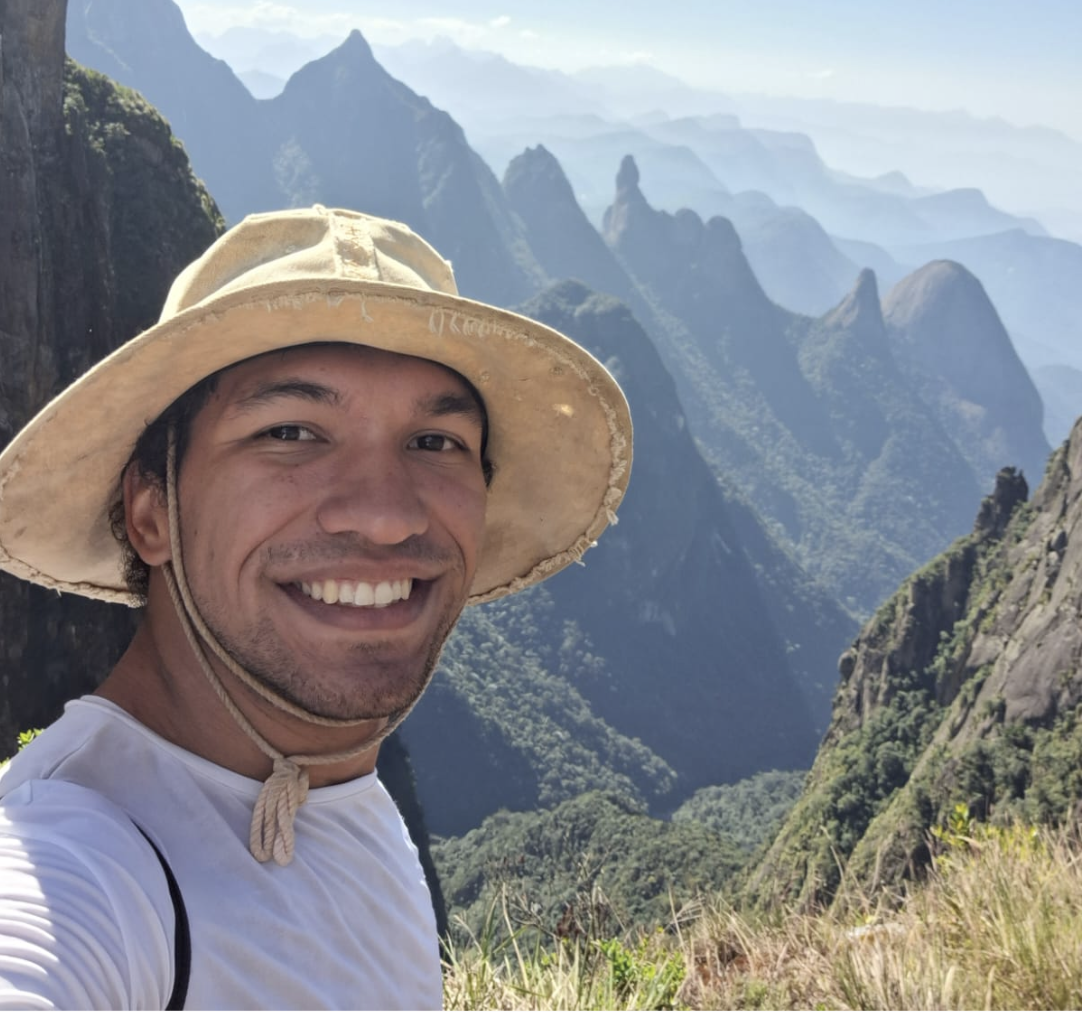
\includegraphics[width=0.5\linewidth]{figs/gabriel_picture} \end{center}

\textbf{Gabriel Garcia}

Doutorando em ecologia pela USP. Mestre em Ecologia pela UnB e Bacharel em Biologia pela UFRN

\begin{quote}
Participo da EcoEscola porque acredito ser uma oportunidade de unir minha paixão pela ecologia com o desejo de ensinar. Valorizo poder contribuir para a formação dos estudantes, algo que vivenciei em edições anteriores do evento, onde pude ensinar e aprender com pessoas de todo o país, enriquecendo meus próprios conhecimentos.
\end{quote}

\begin{center}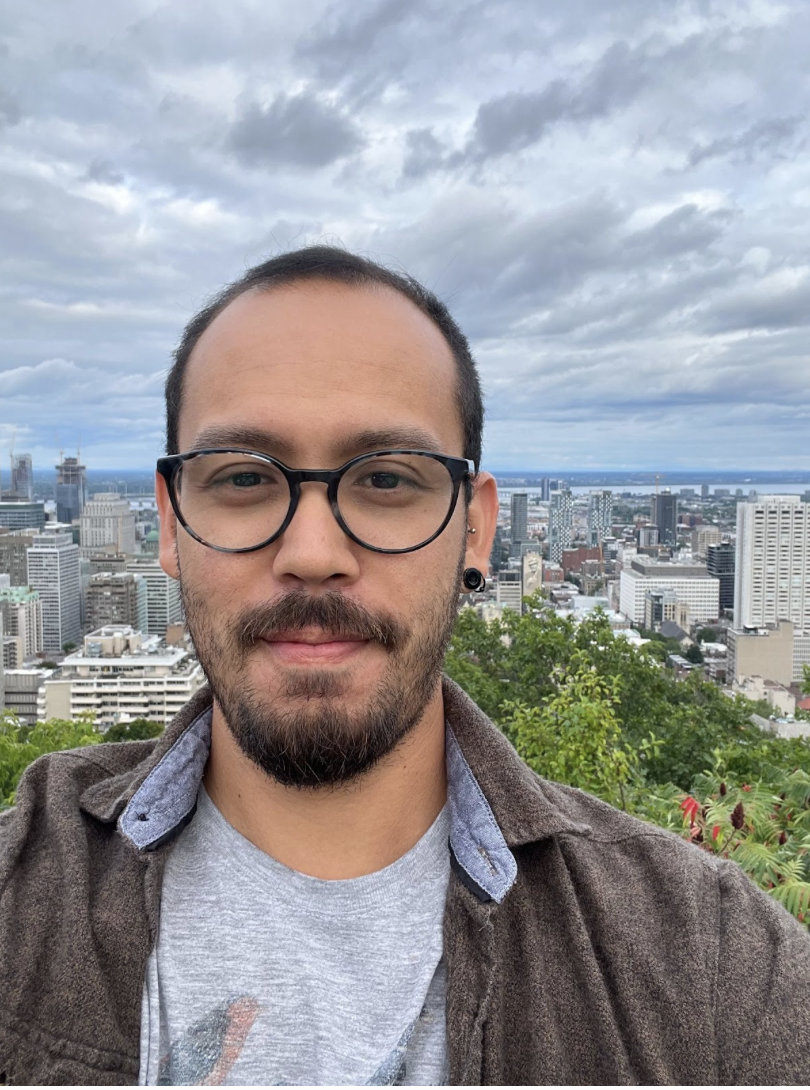
\includegraphics[width=0.5\linewidth]{figs/naka_picture} \end{center}

\textbf{Gabriel Nakamura}

Pós-doutorando no Laboratório de Macroevolução e Macroecologia - USP

\begin{quote}
Sou licenciado em Biologia, e o ensino sempre ocupou uma parte importante e prazerosa na minha carreira acadêmica. Vejo na EcoEscola uma oportunidade para que eu possa contribuir na formação de estudantes em Ecologia.
\end{quote}

\begin{center}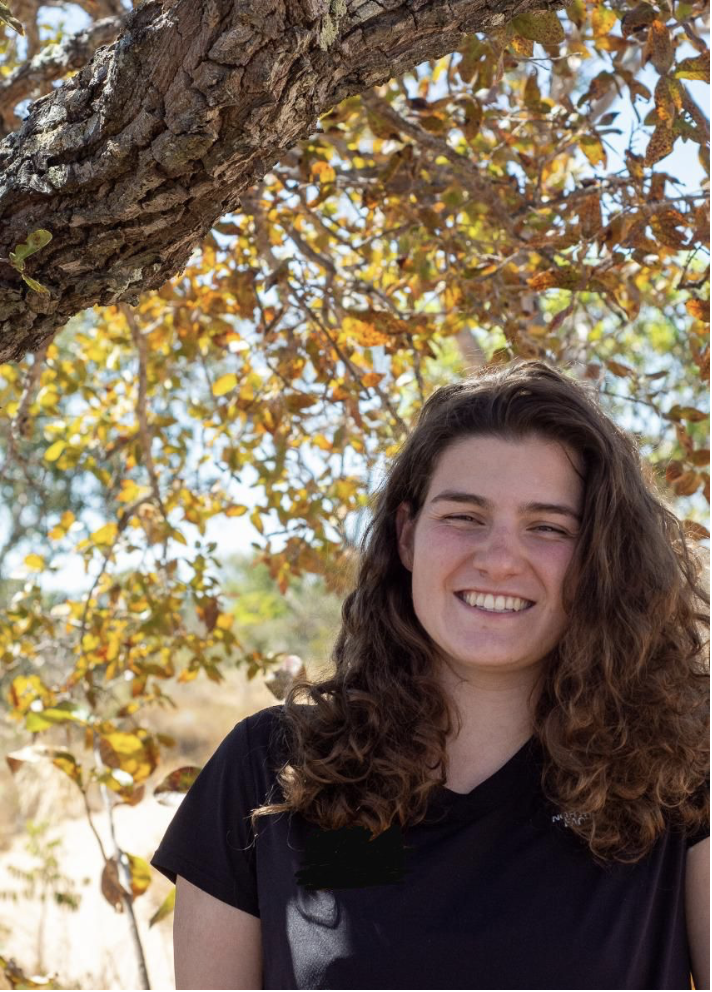
\includegraphics[width=0.5\linewidth]{figs/gabi_picture} \end{center}

\textbf{Gabriela Longo}

Mestranda do Programa Interunidades no Ensino de Ciências (PIEC-USP).

\begin{quote}
Gosto muito de projetos de extensão universitária, e acredito que o ensino, a pesquisa e a extensão de fato só fazem sentido se caminharem juntos. Vejo na EcoEscola uma oportunidade de pensar e atuar nessas três esferas.
\end{quote}

\begin{center}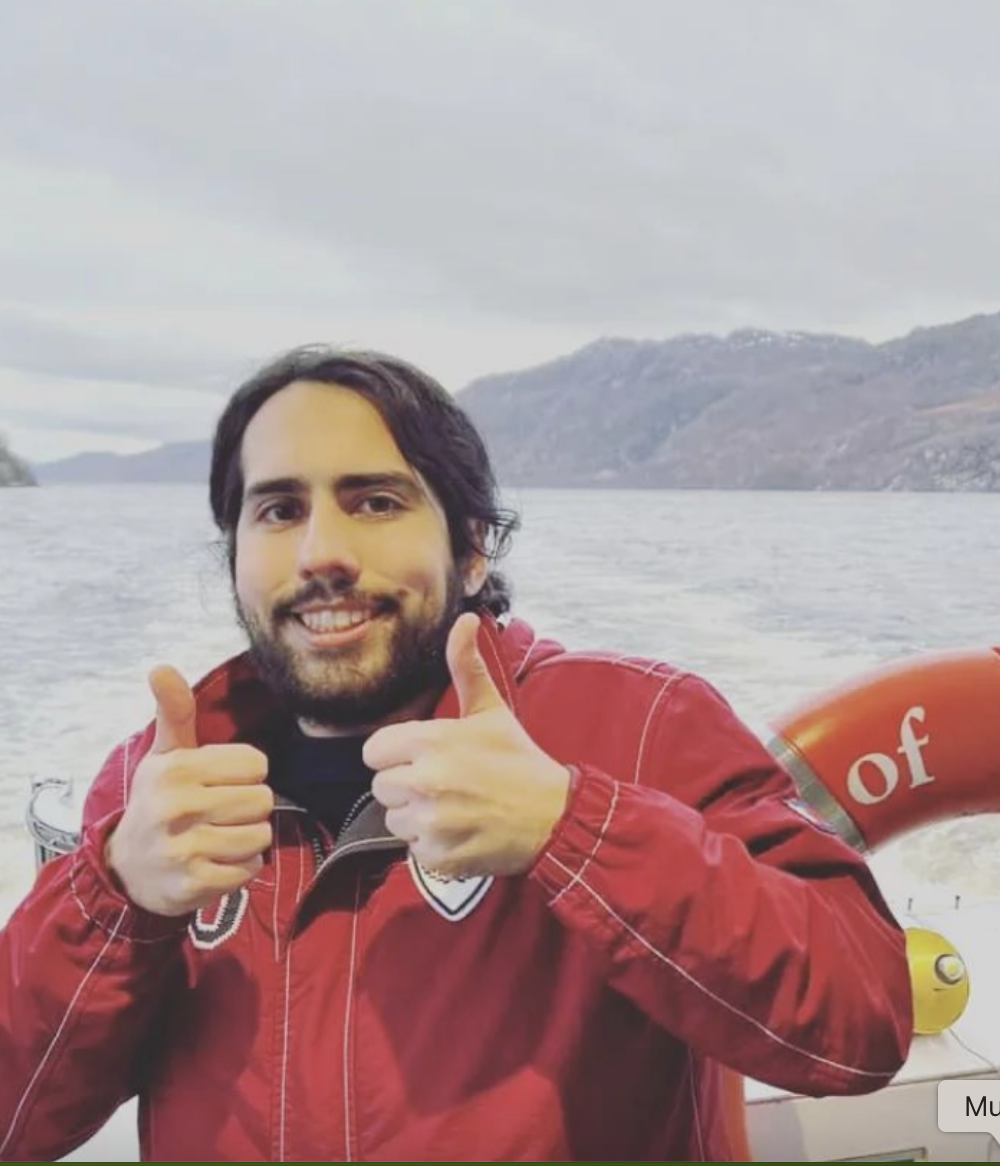
\includegraphics[width=0.5\linewidth]{figs/lucas_picture} \end{center}

\textbf{Lucas Freitas}

Mestre e atual Doutorando em Ecologia no Laboratório de Ecologia Teórica USP

\begin{quote}
``Me interessei pelo projeto pelo seu caráter de divulgação da Ecologia como ciência em seus mais diversos aspectos.''
\end{quote}

\begin{center}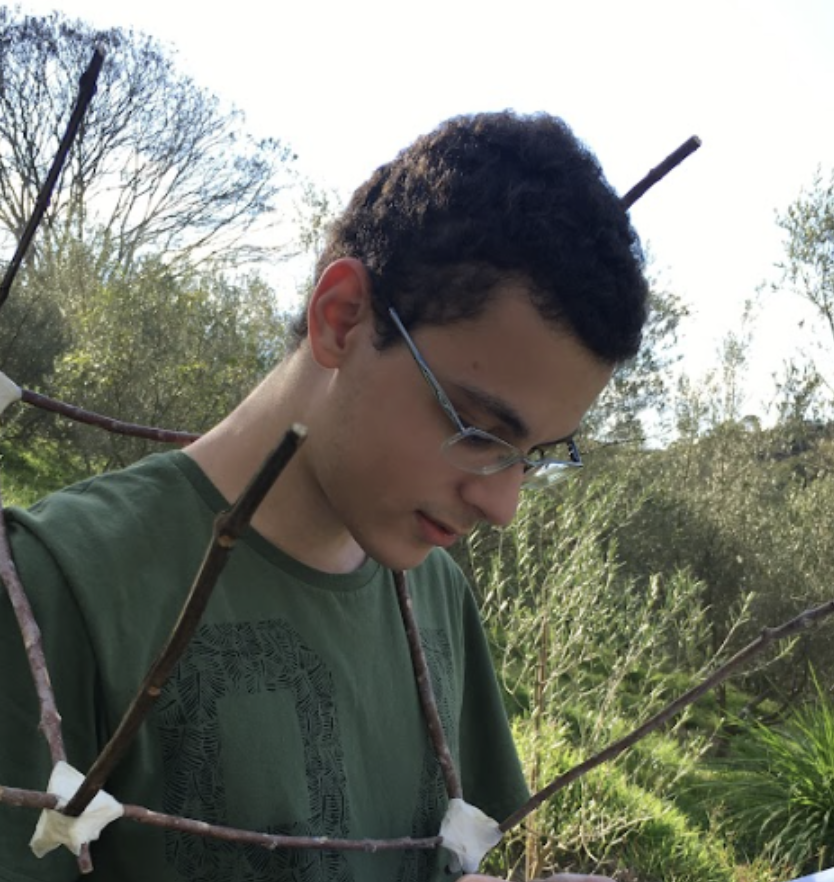
\includegraphics[width=0.5\linewidth]{figs/pepe_picture} \end{center}

\textbf{Matheus Pepe}

Mestre em Ecologia no Laboratório de Ecologia de Florestas Tropicais.

\begin{quote}
Eu sempre gostei de fazer parte de vários projetos de extensão universitária no bacharelado. A EcoEscola foi mais uma oportunidade pra não só conseguir participar do meio universitário nesse quesito, mas também oferecer uma experiência legal para outros alunos de como a Ecologia é um campo extremamente enriquecedor.
\end{quote}

\begin{center}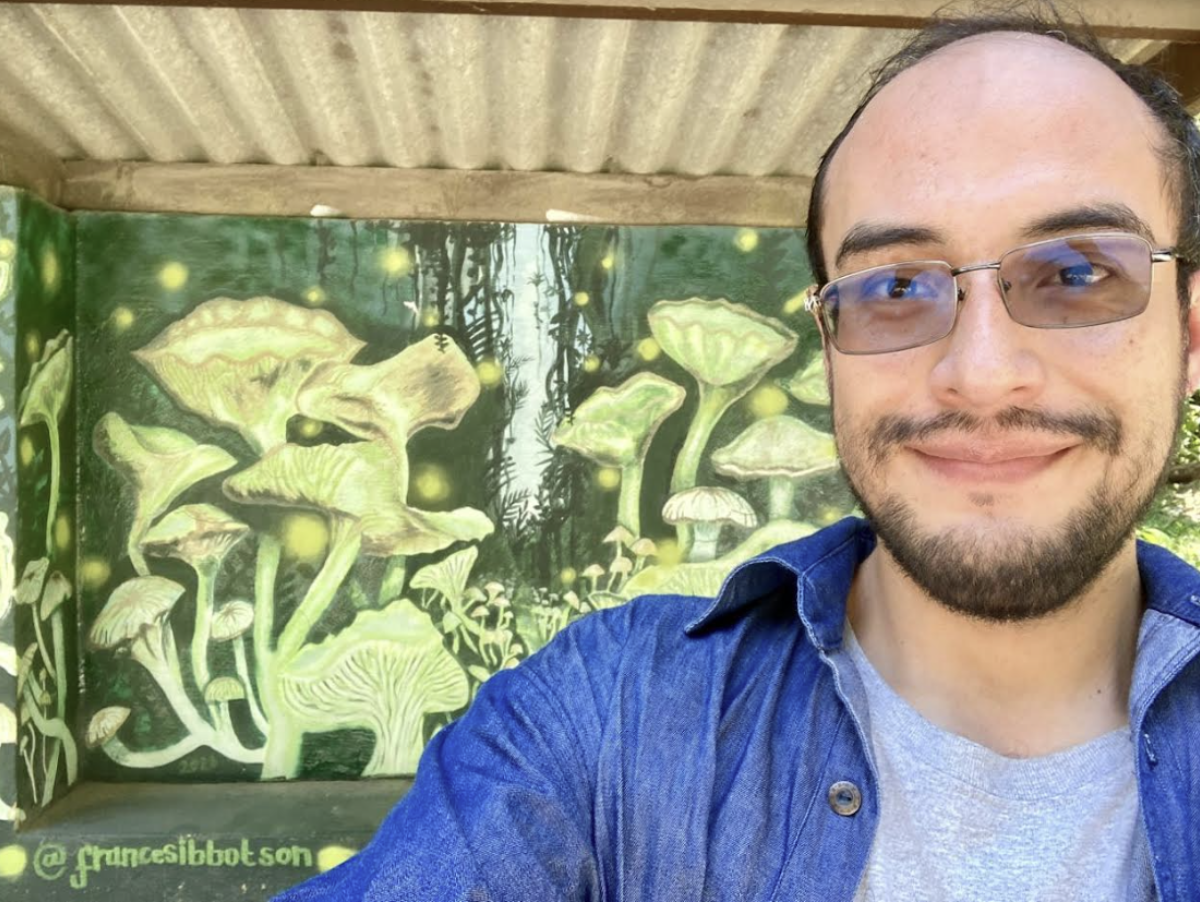
\includegraphics[width=0.5\linewidth]{figs/andres_picture} \end{center}

\textbf{Andres Arguelles}

Pos-doutorando no LAGE-USP e doutorado em Ecologia na UNAM (México)

\begin{quote}
Estou interessado no projeto porque gosto de fazer ecologia e divulgação da ecologia de fungos. Achei muito interessante a dinâmica da EcoEscola, garantindo uma experiência incrível.
\end{quote}

\chapter{Participantes da 6ª EcoEscola}\label{participantes-da-6uxaa-ecoescola}

A 6ª EcoEscola contou com a participação de XX estudantes de XX Universidades do Brasil. Dentre os participantes tivemos XX professores no primeiro módulo do curso, e XX no segundo módulo. A seguir a lista completa dos participantes da 6ª EcoEscola

\chapter{Os projetos}\label{os-projetos}

Nesta edição (6ª EcoEscola) decidimos compartilhar os resumos dos projetos desenvolvidos durante o Módulo 2 acreditando que este material irá servir para duas finalidades principais. Primeiro, para a divulgação dos trabalhos científicos realizados pelos estudantes. Segundo, para que possa fornecer inspiração para práticas de pesquisa e ensino em ecologia.

Os estudantes foram divididos em cinco grupos. Cada grupo ficou responsável pelo desenvolvimento de um projeto proposto por um orientador. Os projetos a serem desenvolvidos durante o módulo 2 foram selecionados a partir de um conjunto de propostas enviadas por estudantes de mestrado e doutorado que demonstraram interesse em orientar durante a fase prática da EcoEscola. Cinco projetos foram selecionados baseado na sua executabilidade, complementariedade de temas e clareza das questõdes propostas. Estes projetos foram discutidos previamente entre os membros da comissão organizadora e ajustados em conjunto com os orientadores de cada grupo. Os grupos e seus orientadores foram os seguintes:

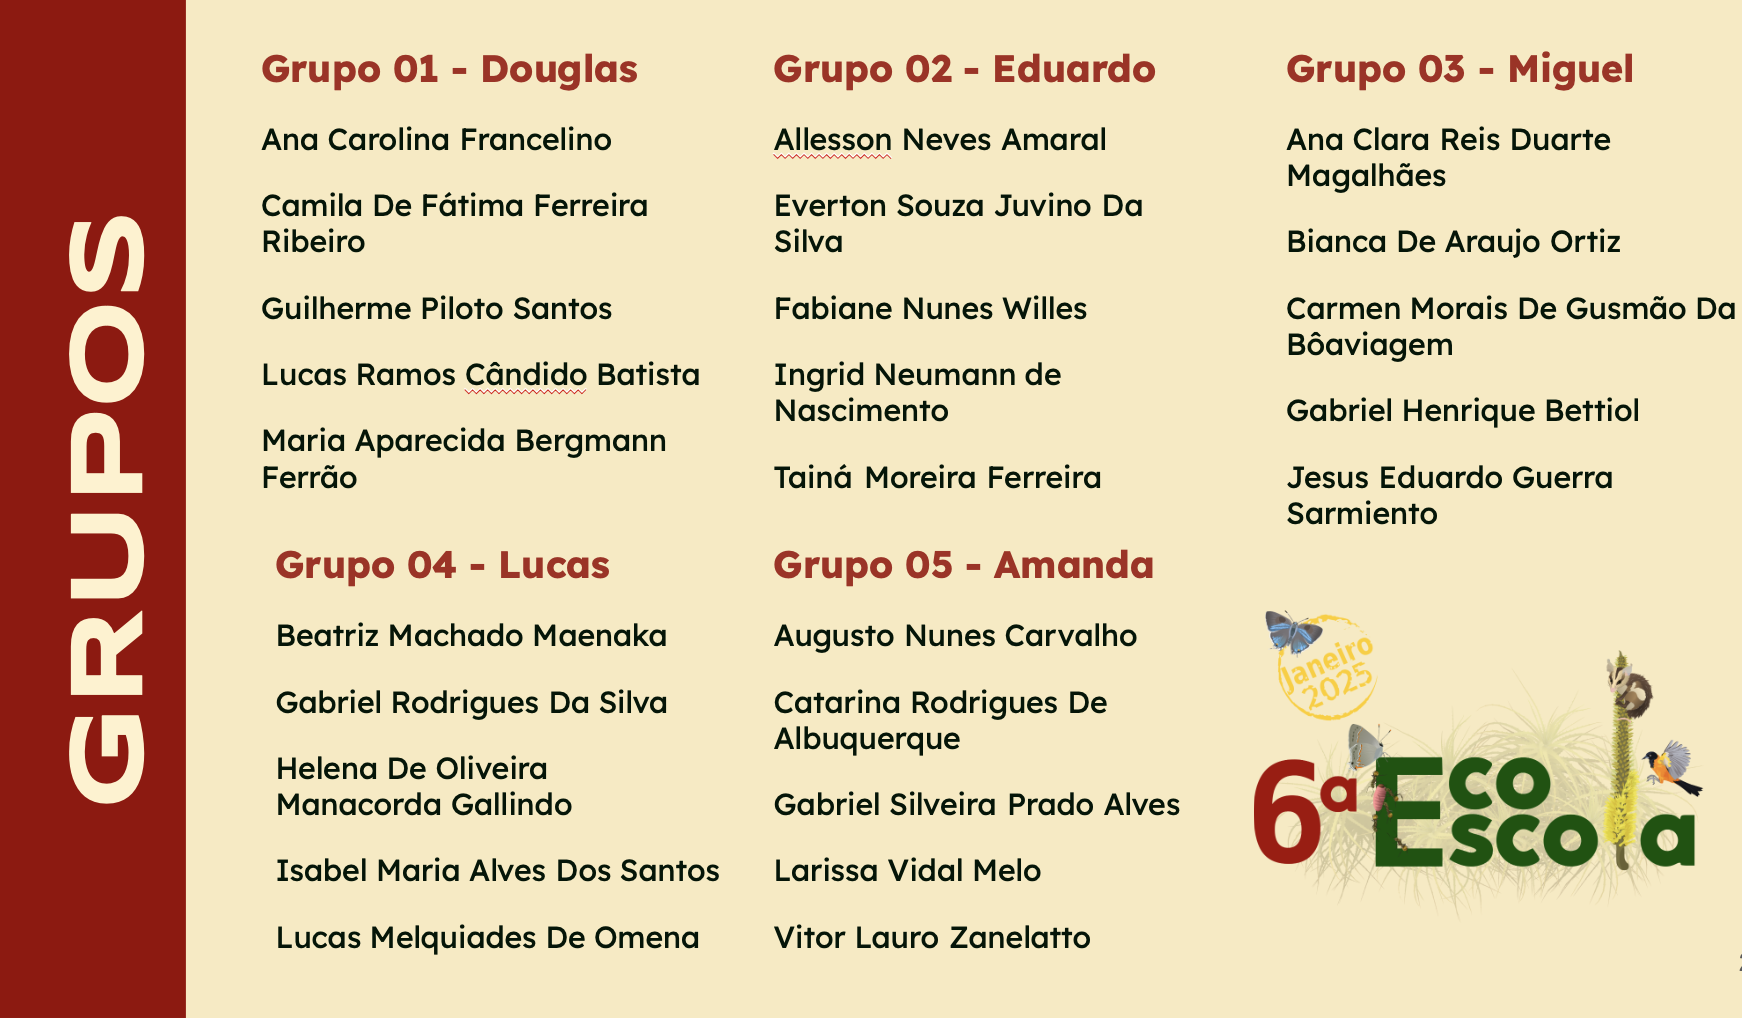
\includegraphics[width=8.06in]{figs/grupos_modulo2}
Grupos e orientadores da 6ª EcoEscola

Os estudantes realizaram todas as fases do projeto de pesquisa, incluindo a coleta de dados, análises, escrita de resumo e apresentação.

\begin{center}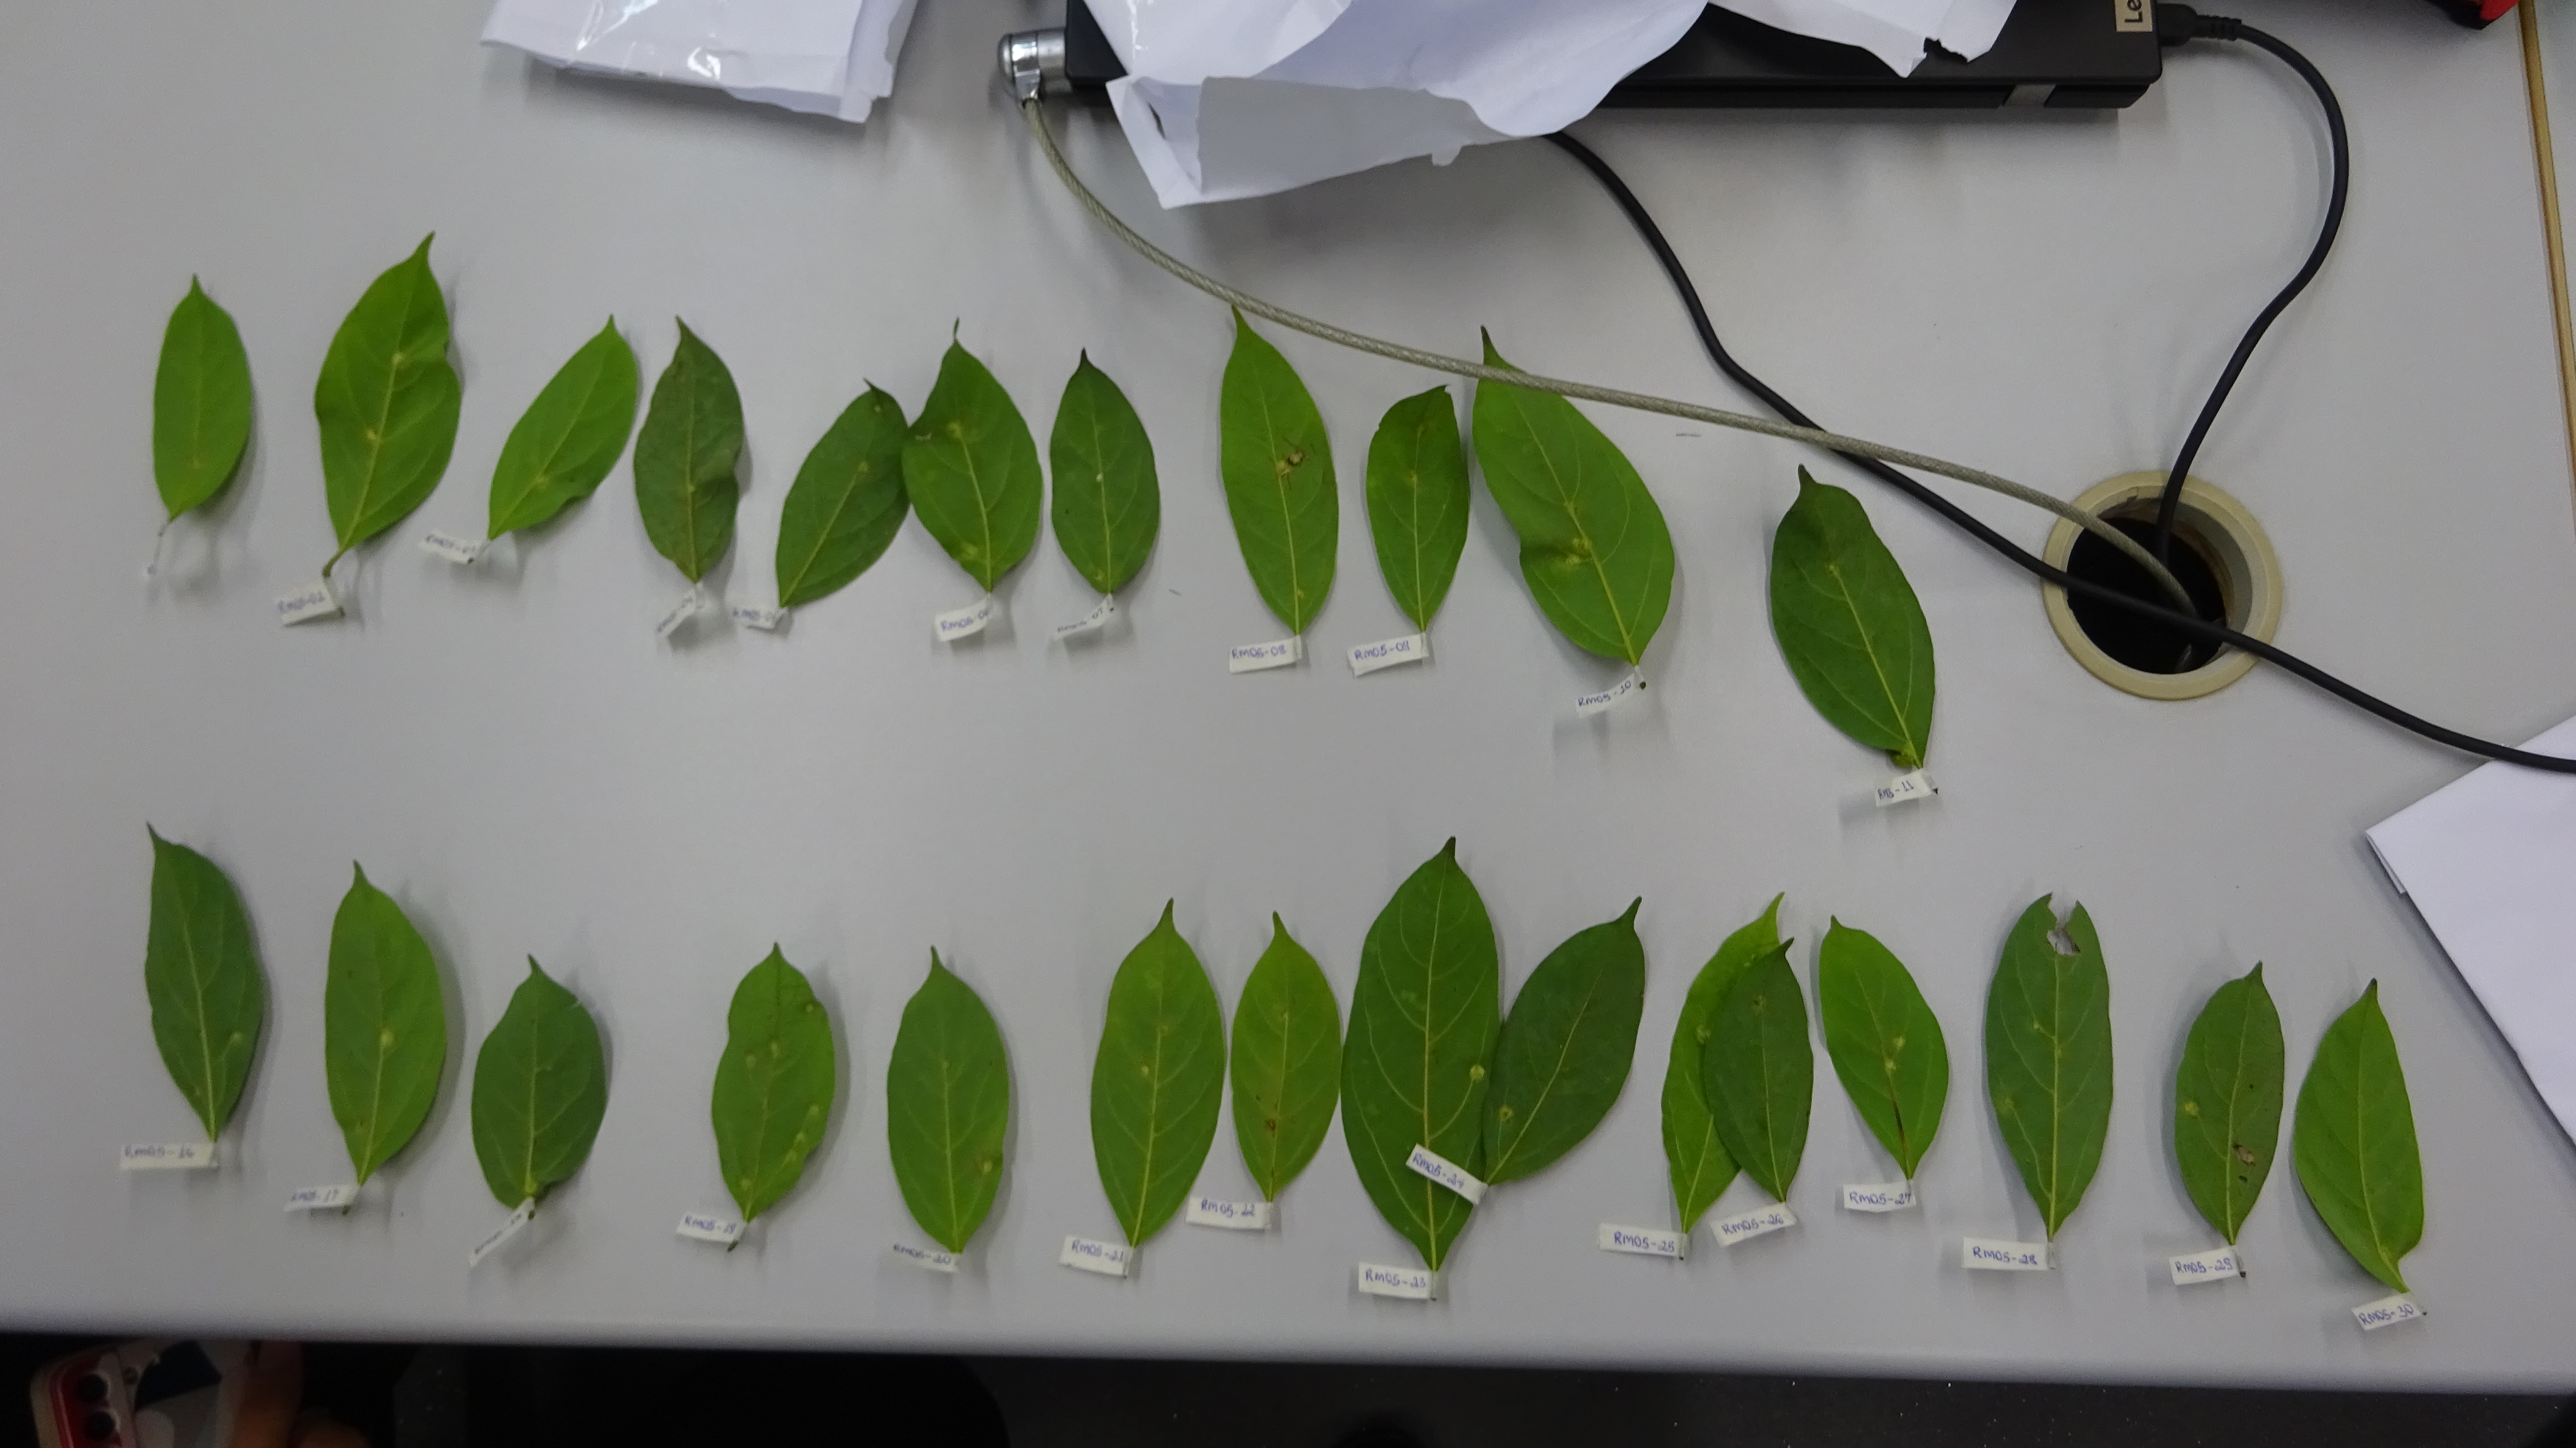
\includegraphics[width=0.7\linewidth]{figs/coleta1} \end{center}

Coleta de dados

\begin{center}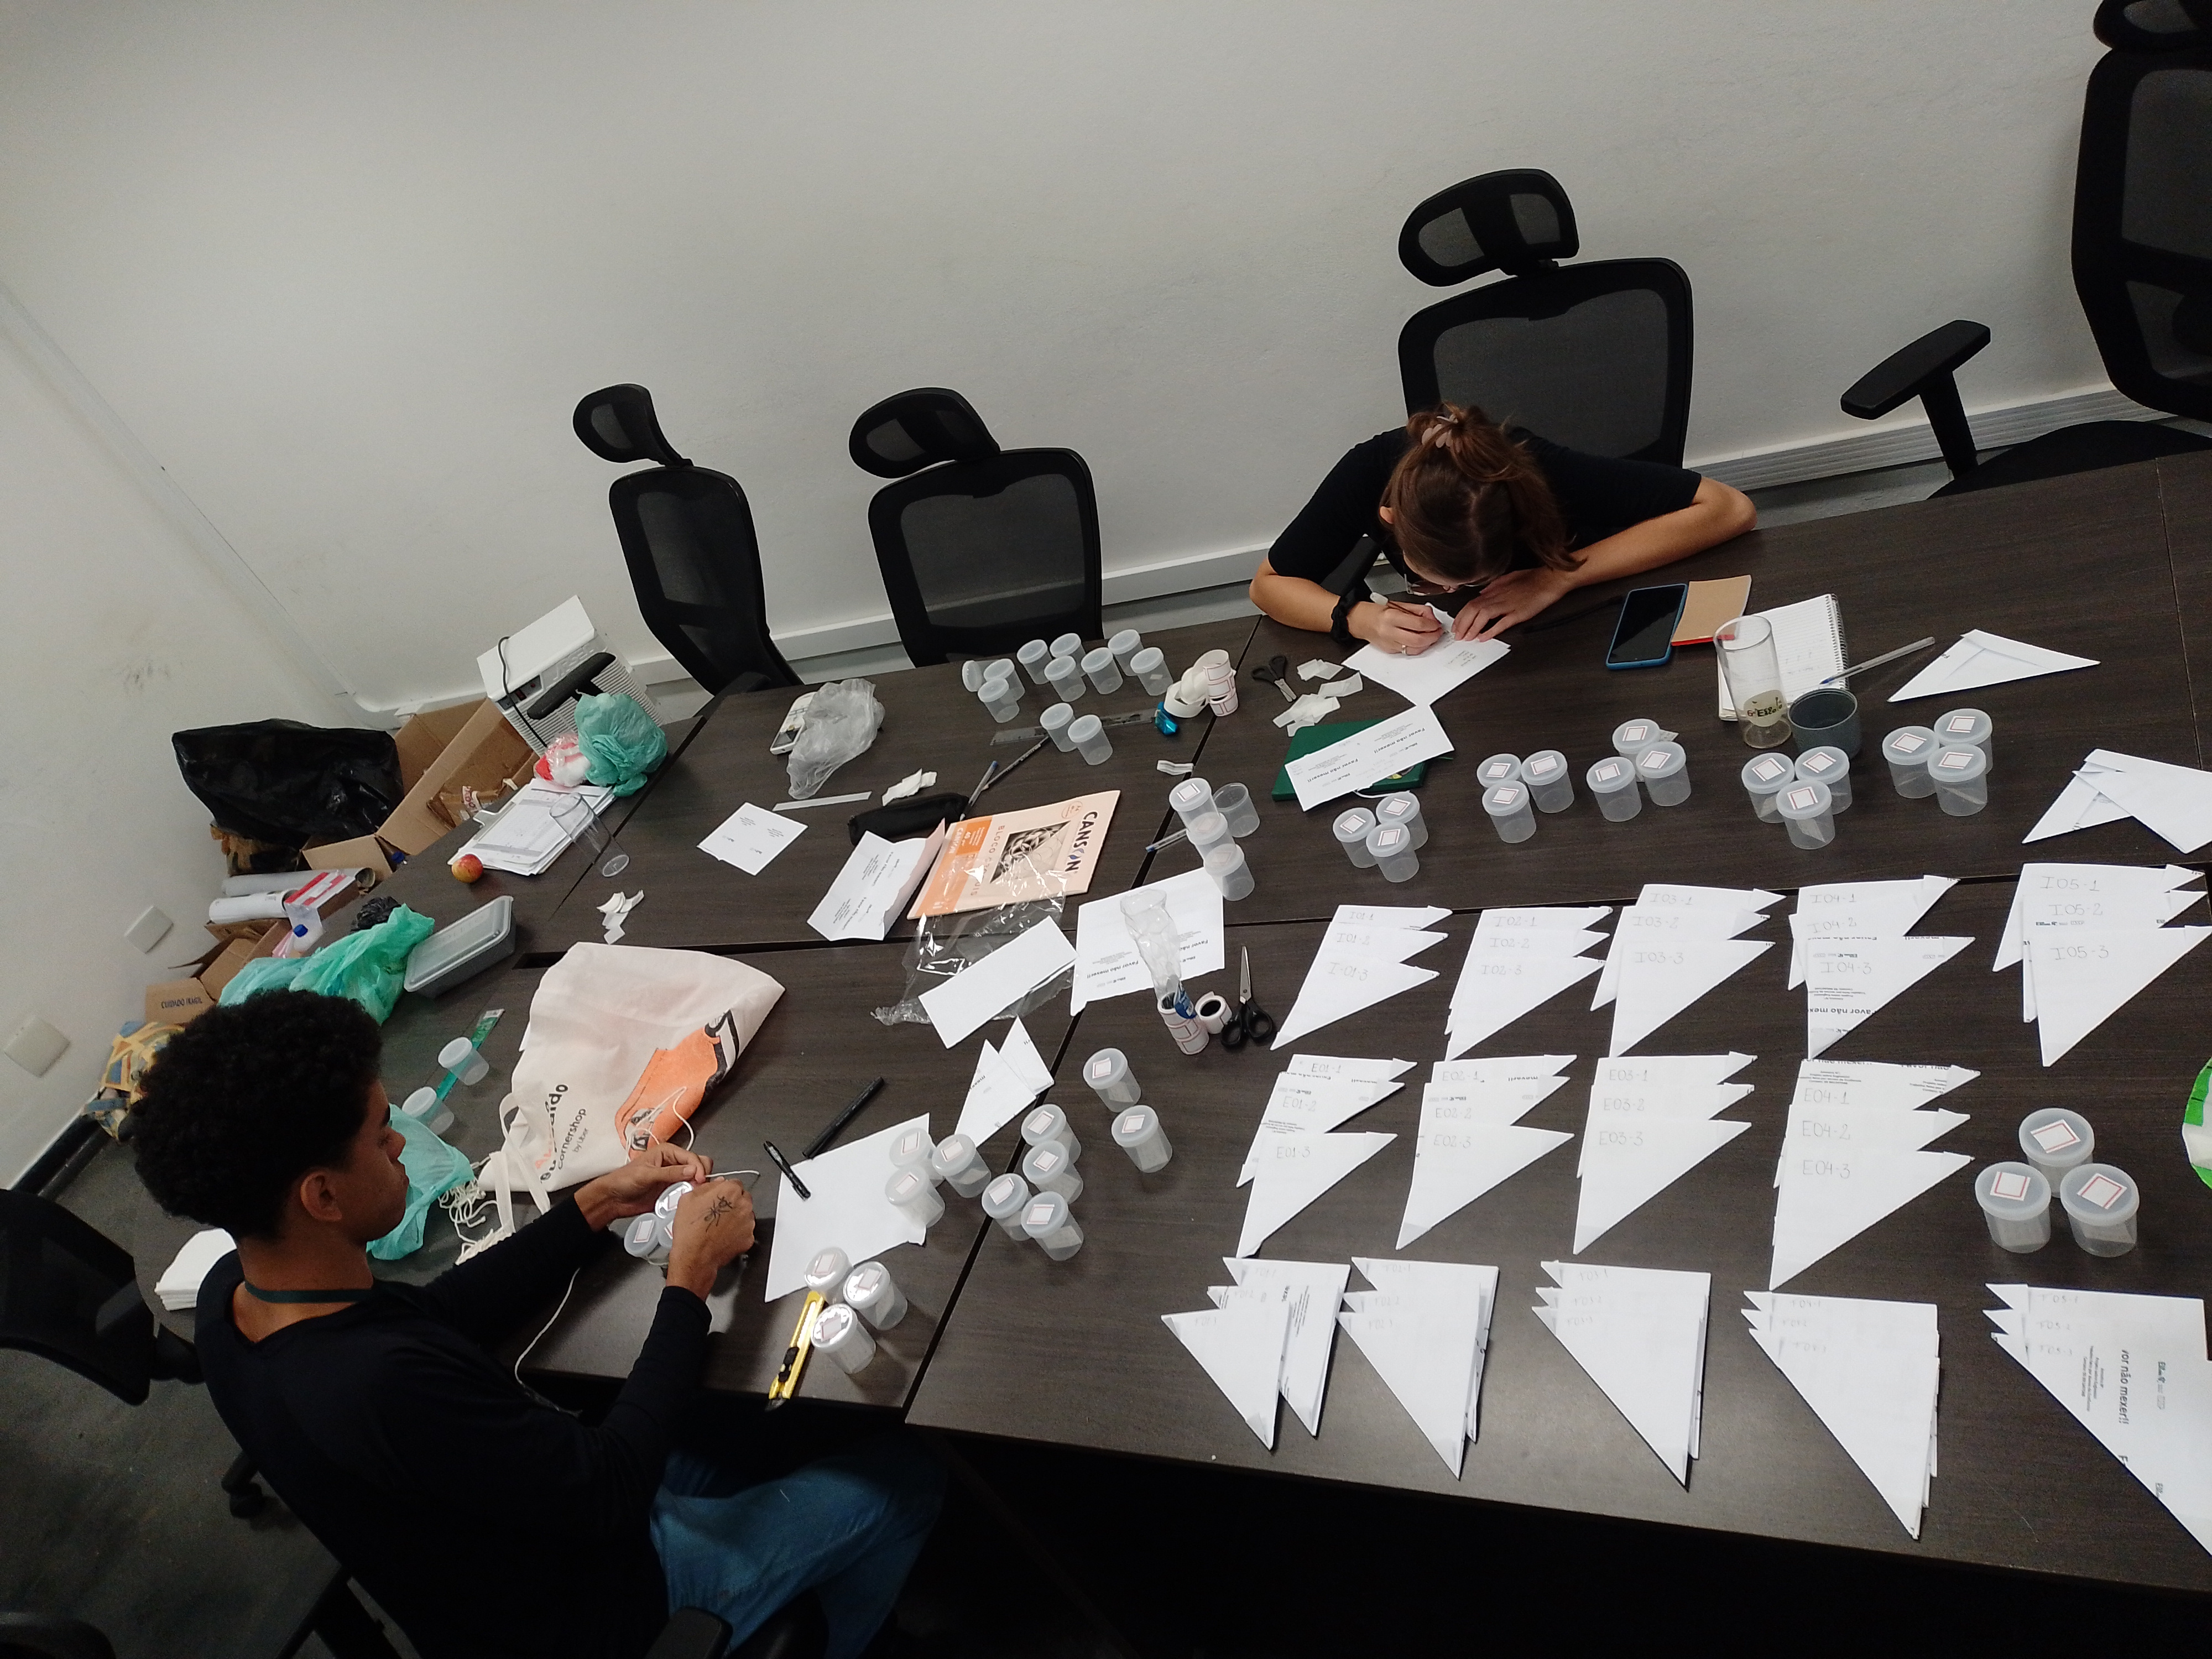
\includegraphics[width=0.7\linewidth]{figs/coleta2} \end{center}

\begin{center}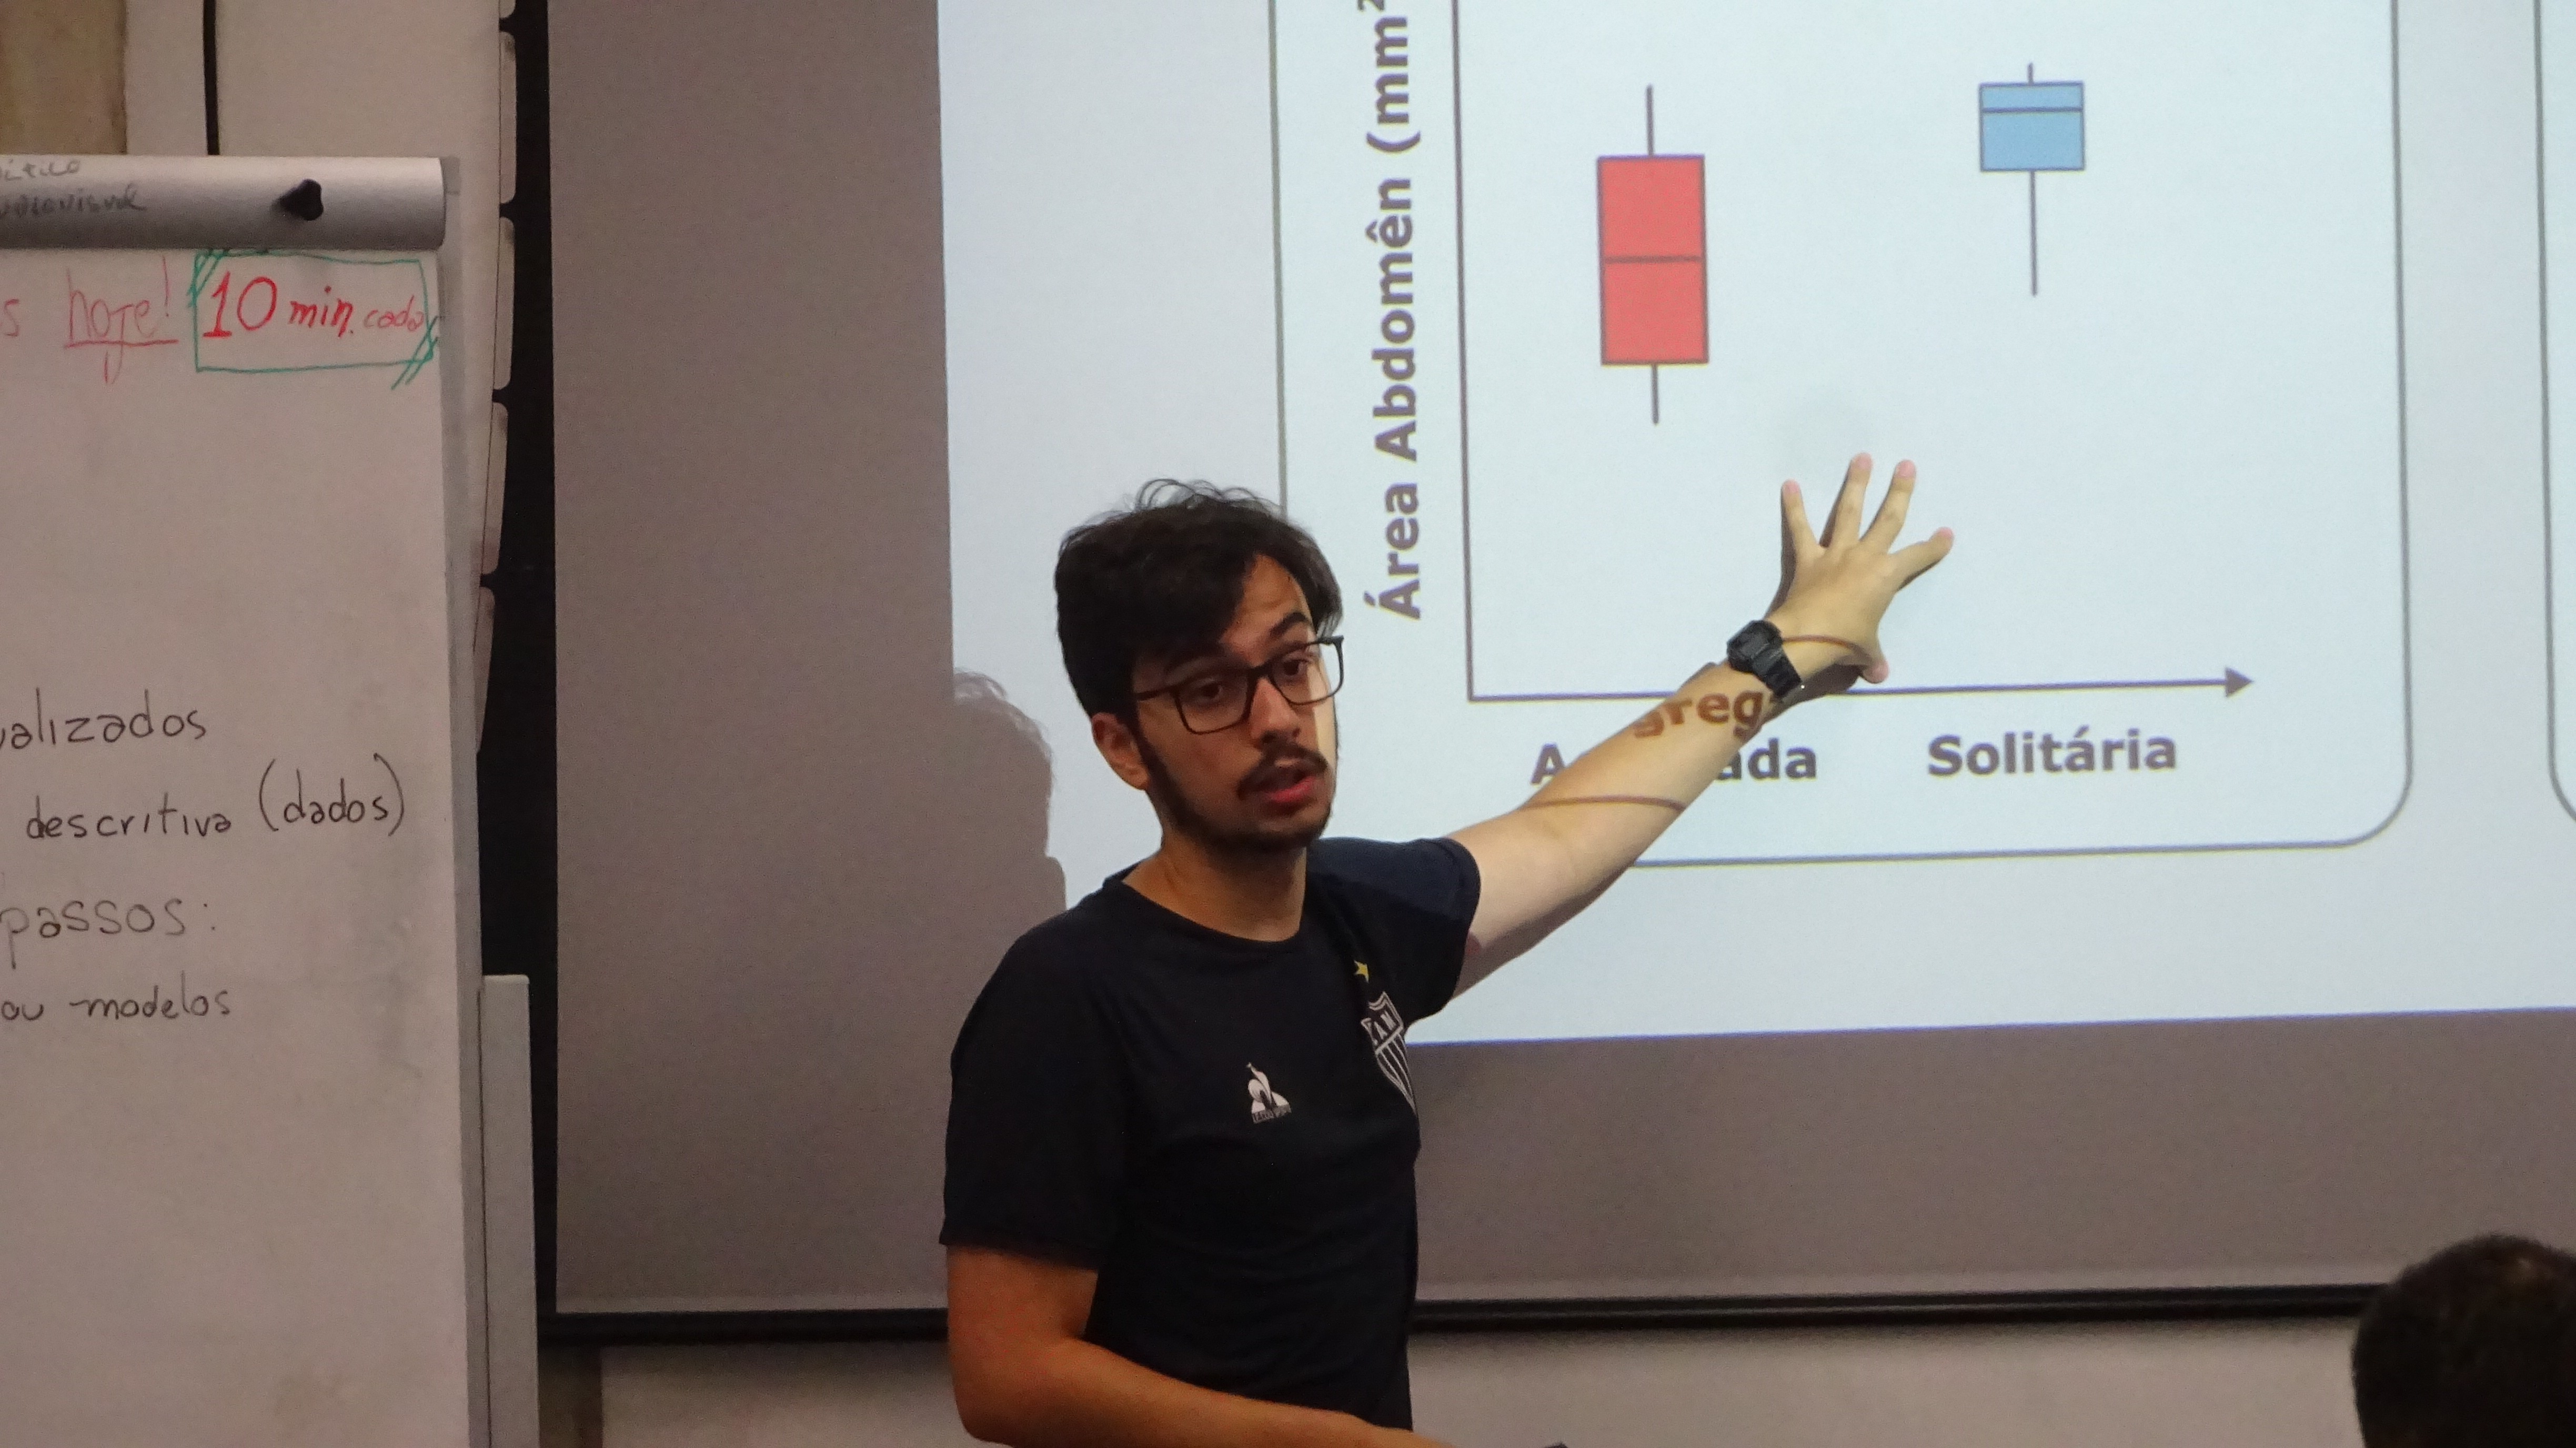
\includegraphics[width=0.7\linewidth]{figs/apresentacao1} \end{center}

Apresentação dos resultados

\chapter{\texorpdfstring{Cobertura e dominância de samambaias epífitas em \emph{Tipuana tipu}}{Cobertura e dominância de samambaias epífitas em Tipuana tipu}}\label{cobertura-e-dominuxe2ncia-de-samambaias-epuxedfitas-em-tipuana-tipu}

\begin{quote}
Grupo 1: Francelino, A.C., Ribeiro, C.F.F., Santos, G.P., Batista, L.R.C., Bergmann, M.A.~e Cirino, D.W.
\end{quote}

\begin{quote}
Orientador: Douglas William Cirino
\end{quote}

Plantas pteridófitas utilizam árvores como forófitos, representando uma interação interespecífica neutra, onde não há prejuízos à planta hospedeira. Nessa interação, o espaço nos galhos do forófito é um importante recurso, gerando competição entre epífitas, com cenários de dominância ou coexistência, a depender do ambiente. O objetivo deste trabalho foi compreender se há relação dos microclimas com a cobertura e a coexistência de pteridófitas epífitas no forófito Tipuana tipu (Benth.) Kuntze. Nossa hipótese é que a dominância da epífita Microgramma sp. em relação a outras pteridófitas é menor em cenários de microclima mais favorável. Além disso, supomos que quanto maior o índice de vegetação maior será a cobertura vegetal total de epífitas nos galhos de Tipuana tipu. Amostramos 40 indivíduos do forófito sob diferentes condições microclimáticas. Fotografamos quadrantes de 50x50 cm, a diferentes alturas na face sul de cada Tipuana tipu (Benth.) Kuntze. Estimamos as áreas de cobertura de três morfotipos de pteridófitas mais comuns. Calculamos a dominância de Microgramma sp. sobre outras epífitas como uma proporção da área total coberta por epífitas em cada galho amostrado. Calculamos o índice normalizado de vegetação (NDVI) utilizando ortofotos de 1m de resolução e medimos o NDVI médio dentro de buffers de 25, 50 e 100m de raio a partir do forófito. Testamos nossas hipóteses utilizando a função betareg do software R (V 4.4.2). Nosso resultado demonstra que quanto maior a média do NDVI nos buffers de 25 e 50m menor será a dominância da Microgramma sp. (p=0,010 e p=0,026, respectivamente), corroborando nossa hipótese, enquanto não houve diferença estatística no buffer de 100m (p=0,153). Adicionalmente, não houve relação estatística entre o NDVI e a cobertura das epífitas (p\textgreater0,05). Isso pode indicar que o microclima pode não ser o fator principal influenciando essa ocupação, refutando nossa segunda hipótese. Por outro lado, pudemos confirmar que o microclima é preponderante na dominância de Microgramma sp. sobre as outras samambaias epífitas, uma vez que em raios menores o efeito é significativo e em raios de 100m o efeito desaparece. Estudos anteriores afirmam que a interação entre epífitas com diferentes formas de dispersão pode ser negativa1, Microgramma sp. é a única epífita trepadeira amostrada, podendo ser dominante, mas em microclimas mais favoráveis a competição pode ser mais intensa. Como hipótese a posteriori, corroboramos que quanto maior a altura da amostra no forófito maior será a cobertura de epífitas (p=0,001), como já observado anteriormente². Os resultados obtidos auxiliam a compreender como o microclima pode influenciar na dominância entre as pteridófitas epífitas, e entender fatores que alteraram o epifitismo e competição.

\textbf{Palavras-chave:} Coexistência; microclima; Microgramma sp; pteridófitas epífitas

\chapter{Efeito da paisagem na comunidade de Euglossini em diferentes fragmentos}\label{efeito-da-paisagem-na-comunidade-de-euglossini-em-diferentes-fragmentos}

\begin{quote}
Allesson Neves; Everton Juvino; Fabiane Willes; Ingrid Neumann; Tainá Ferreira
\end{quote}

\begin{quote}
Orientador: Eduardo Moreira
\end{quote}

A composição da paisagem influencia diretamente a diversidade biológica. Em paisagens complexas, espera-se maior diversidade de nichos, o que favorece a coexistência de diferentes espécies. Cenários mais heterogêneos também oferecem mais opções de abrigo e refúgio. A diversidade da tribo Euglossini, fundamental para a polinização, é afetada por variáveis estruturais da paisagem, que influenciam tanto a disponibilidade de recursos quanto a dinâmica populacional das espécies. Esse grupo, com distribuição vertical heterogênea, é considerado um bom indicador da diversidade e complexidade da paisagem devido aos seus diversos modos de vida. Investigamos a relação entre a heterogeneidade ambiental, a proporção de vegetação e a abundância e riqueza de Euglossini, com a hipótese de que paisagens mais heterogêneas e vegetadas favorecem maior diversidade. Realizamos coletas com armadilhas de cheiro contendo eucaliptol, distribuídas em 14 pontos ao longo de um gradiente de composições de paisagem na Universidade de São Paulo - Campus Butantã e arredores, entre 07 e 10 de fevereiro de 2025. Triamos e identificamos as abelhas até o nível de espécie. A análise da paisagem foi realizada por meio de imagens de satélite (Sentinel 1, Sentinel 2 e Alos Palsar), classificadas utilizando o algoritmo Random Forest. Para a análise, foram utilizados o índice de Shannon-Wiener e a proporção de vegetação. Modelos de regressão linear foram desenvolvidos, com riqueza e abundância de Euglossini como variáveis resposta, e o índice de Shannon e a proporção de vegetação como variáveis explicativas. Capturamos 198 indivíduos, distribuídos nos gêneros Eulaema (125 indivíduos), Euglossa (71) e Exaerete (2), totalizando 10 espécies, sendo as mais representativas Eulaema nigrita (63,13\%), Euglossa carolina (17,17\%) e Euglossa solangeae (15,15\%). Embora os modelos de regressão não tenham mostrado valores de p significativos, observou-se uma tendência de aumento na riqueza e abundância de Euglossini em locais com maior proporção de vegetação. Este estudo destaca a importância de avaliar o impacto das alterações na paisagem sobre a riqueza de espécies. Estudos com mais eventos amostrais e por períodos mais longos são necessários para fortalecer os resultados.
\textbf{Palavras-chave}: Heterogeneidade; Diversidade de polinizadores; Composição; Estrutura da paisagem; Métricas espaciais;

\chapter{O efeito da disponibilidade de recursos na distribuição de galhas foliares}\label{o-efeito-da-disponibilidade-de-recursos-na-distribuiuxe7uxe3o-de-galhas-foliares}

\begin{quote}
Ana Clara Reis Duarte Magalhães¹, Bianca de Araújo Ortiz2, Carmen Morais de Gusmão da Bôaviagem³, Gabriel Henrique Bettiol4 e Jesus Eduardo Guerra Sarmiento5
\end{quote}

\begin{quote}
Orientador: Miguel Piovesana Pereira-Romeiro
\end{quote}

A disponibilidade de recursos pode influenciar a distribuição espacial dos seres vivos em diferentes escalas. Folhas podem ser encaradas como microhabitats heterogêneos, apresentando variação na disponibilidade de recursos alimentares. Insetos galhadores dependem dos recursos da folha (seiva) e, portanto, devem selecionar seu local de fixação a partir deste sinal. Temos como objetivo compreender o papel da disponibilidade de recursos na distribuição de galhas foliares. Esperamos que haja preferência pela base da nervura central (BNC) por ser uma região de maior concentração de seiva (tanto bruta quanto elaborada) quando comparado com outras regiões inervadas. Coletamos 30 folhas galhadas de 12 indivíduos (N=360) de Lauraceae na Rua do Matão (USP-Butantã). Subamostramos 77 folhas e quantificamos (I) a área de nervuras, (II) área da BNC e a presença de galhas (III) nas nervuras e (IV) da BNC. Para verificar a preferência de insetos galhadores pela BNC, realizamos um teste de Qui-Quadrado de aderência para comparar a frequência observada de folhas com galhas na BNC contra a frequência esperada. Para obter o número esperado de folhas com galhas na BNC e também nas demais nervuras, multiplicamos as médias das proporções da área da BNC e da área das demais nervuras pelo número de amostras, respectivamente. Observamos 5 folhas com galhas na BNC (esperado = 6,09) e 77 com galhas nas demais nervuras (esperado = 70,9). Não houve preferência das galhas pela BNC em relação às demais nervuras da folha (X²=0,37; p=0,054). Ainda que a BNC possua maior quantidade de recursos, sua área disponível é significativamente menor e, portanto, podemos esperar que ela rapidamente atinja uma capacidade de suporte. É possível que as ninfas prefiram selecionar outras nervuras da folha para evitar a competição por espaço e recurso na BNC às custas de recursos reduzidos. Alternativamente, é possível que a oviposição aconteça quando as folhas ainda são jovens. Neste estágio, as nervuras do ápice foliar estão mais maduras que as da BNC (desenvolvimento basípeto). Dessa forma, pode haver uma preferência das ninfas por áreas mais desenvolvidas, independente do padrão de nervação observado numa folha adulta. Estes processos podem ser alguns dos que explicam o padrão observado. Não podemos afirmar que haja algum mecanismo de escolha de posição da galha em relação aos recursos disponíveis na folha. Ressaltamos a necessidade de mais estudos deste tipo, considerando que os mecanismos de indução de galha ainda são pouco estudados, especialmente nos neotrópicos.

\textbf{Palavras-chave}: Psylloidae; nervação foliar; parasitismo; interação inseto-planta; Lauraceae

\chapter{A influência da escolha do recurso alimentar sobre o fitness em besouros brocadores}\label{a-influuxeancia-da-escolha-do-recurso-alimentar-sobre-o-fitness-em-besouros-brocadores}

\begin{quote}
Beatriz M. Maenaka, Gabriel R. Silva, Helena Gallindo, Isabel Alves, e Lucas Melquiades, Lucas Freitas
\end{quote}

\begin{quote}
Orientador: Lucas Freitas e Gabriel Nakamuram
\end{quote}

Os organismos são selecionados para otimizar a obtenção de energia e minimizar os custos associados à manipulação de recursos, aumentando as chances de sobrevivência e sucesso reprodutivo. Os besouros brocadores (e.g., Bruchidae) possuem um ciclo de vida parasitoide, colocando ovos na superfície externa de frutos, que fornecem abrigo e nutrientes para o desenvolvimento das larvas. Ao eclodirem, as larvas deixam cavidades circulares na superfície do fruto. Este estudo testou como a escolha de recursos alimentares afeta a aptidão da prole. Segundo a teoria de forrageamento ótimo, esperamos que larvas com maior aptidão estejam associadas a frutos com mais recursos, enquanto larvas com menor aptidão seriam associadas a frutos com maior custo energético de manipulação. Para testar essa hipótese, coletamos frutos caídos ao redor das palmeiras do Jardim Japonês da USP. Medimos o volume dos frutos com paquímetro (precisão de 0,01 mm), utilizando a fórmula do cilindro, e a espessura da casca para quantificar o custo de manipulação. Como medida de aptidão, analisamos o diâmetro da cavidade de saída das larvas. Trabalhamos com 100 frutos, e para evitar efeitos de confusão devido ao uso compartilhado do recurso por diferentes espécies, visualizamos a distribuição do diâmetro das cavidades com um histograma. Ao identificar uma distribuição bimodal, excluímos frutos com cavidades menores que 2,5 mm (n = 16), assumindo que pertenciam a outra espécie de besouro. Os frutos com cavidades maiores ou iguais a 2,5 mm (n = 84) foram analisados. Testamos os efeitos do volume do fruto e da espessura da casca sobre o diâmetro da cavidade de saída das larvas com regressões lineares. O volume do fruto influenciou positivamente a aptidão (R² = 10,03\%, p = 0,01, coeficiente angular = 0.12), mas a espessura da casca não teve efeito significativo (R² = -0,001\%, p = 0,35, coeficiente angular = -0.05), indicando que o custo de manipulação da casca não limita a aptidão. Não encontramos interação significativa entre volume e espessura da casca (R² = 11,57\%, p = 0,02), destacando a importância da quantidade de recursos na aptidão das larvas. Nossos resultados indicam que o sucesso reprodutivo dos besouros brocadores está relacionado com a disponibilidade de recursos nos frutos, e a baixa importância da espessura da casca sugere que fatores ambientais, como a quantidade de frutos ou a presença de ovos de outros indivíduos, também influenciam a escolha do local de desova.

\textbf{Palavras-chave}: Besouro brocador; trade-off; esforço de manipulação; fitness; forrageamento ótimo.

\chapter{Vizinhar ou não vizinhar, eis a questão}\label{vizinhar-ou-nuxe3o-vizinhar-eis-a-questuxe3o}

\begin{quote}
Grupo 5: Augusto Carvalho, Catarina Albuquerque, Larissa Vidal e Vitor Zanelatto
\end{quote}

\begin{quote}
Orientadora: Amanda Vieira da Silva
\end{quote}

A formação de agregações coespecíficas é um hábito amplamente distribuído em diferentes animais, sendo facultativa ou obrigatória dependendo do grupo. Em espécies que se agregam de modo facultativo, a limitação ao acesso aos recursos pode ser um fator importante na decisão de estar solitário ou agregado. Recursos alimentares, por exemplo, talvez sejam mais facilmente obtidos em agregações, entretanto, a competição intraespecífica por acesso a esses recursos também pode reduzir a chance individual de obtenção de alimento. Além dos recursos alimentares, a chance de encontrar um parceiro sexual pode ser maior em agregações do que para indivíduos que vagueiam solitariamente. Uma espécie que pode ser encontrada tanto de forma solitária quanto em agregações é a aranha de teia dourada Triconephila clavipes (Linnaeus, 1767), sugerindo a existência de demandas conflitantes entre esses dois hábitos. Neste estudo, investigamos se fêmeas em teias agregadas e isoladas apresentam condição nutricional diferentes entre si e também se fêmeas de teias agregadas apresentam maior aptidão sexual que de teias isoladas. Para isso, contabilizamos e categorizamos teias solitárias e agregadas de T. clavipes em um fragmento de Mata Atlântica. Como estimativa da condição nutricional, medimos a área dorsal do abdômen de fêmeas adultas. Para aptidão sexual, calculamos a proporção de fêmeas sem machos nas teias focais. Nós vimos que o número médio de fêmeas por agregação foi cinco. Não encontramos correlação entre a área abdominal das fêmeas e a agregação ou isolamento das teias. Além disso, a frequência de fêmeas sem machos não diferiu entre os hábitos e, em ambos os casos, a presença de machos foi superior a 70\%. Contrário ao esperado, o hábito de agregação não afeta a condição nutricional e a aptidão sexual das fêmeas. Entretanto, outros mecanismos poderiam explicar os hábitos de agregação das fêmeas. Por exemplo, a limitação de habitats disponíveis resultaria em um processo estocástico de agregação espacial, acarretando na competição entre os indivíduos que compõem uma agregação, de modo que a aptidão individual não seja uniforme dentro dos grupos. Além disso, indivíduos em agregações possuem vantagens na fuga de predadores, a pressão de predação favoreceria a permanência desse hábito na espécie. Os mecanismos exatos que estruturam a distribuição dessa espécie ainda não são claros, evidenciando a relevância de futuras pesquisas acerca da distribuição dos indivíduos, contribuindo na compreensão do comportamento animal e dos processos evolutivos que o moldam.

\textbf{Palavras-chave:} agregação, aptidão sexual; recursos alimentares; distribuição espacial; \emph{Trichonephila clavipes}.

  \bibliography{book.bib,packages.bib}

\end{document}
